% =============================================================================
%  Tài liệu 02 - Đặc tả yêu cầu phần mềm (Software Requirements Specification)
%  Build: latexmk 02-software-requirements-specification.tex   (pdfLaTeX, output in build/)
% =============================================================================
\documentclass[12pt,a4paper]{report}
\usepackage{sumtalk-report}
% =============================================================================
%  sumtalk-info.tex - information shared by every document (01-06).
%  Edit here once; every cover and footer picks it up.
% =============================================================================
\newcommand{\ProjectName}{SumTalk}
\newcommand{\CourseName}{QUẢN LÝ DỰ ÁN PHẦN MỀM}          % cover (upper case)
\newcommand{\CourseNameNormal}{Quản lý Dự án Phần mềm}     % footer
\newcommand{\AcademicYear}{2026 -- 2027}
\newcommand{\Instructor}{\canDien[họ tên giảng viên]}

% One \item per member: "Full name -- student ID", sorted by given name.
\newcommand{\TeamMembers}{%
  \item Nguyễn Anh Duy -- \canDien[MSSV]
  \item Đỗ Thành Đạt -- \canDien[MSSV]
  \item Trần Hải Đăng -- \canDien[MSSV]
  \item Châu Hùng Hào -- \canDien[MSSV]
  \item Bùi Đoàn Minh Nhật -- \canDien[MSSV]
  \item Võ Hoàng Sơn -- \canDien[MSSV]
}


% UI screenshots are taken from the repository, not copied into figures/.
\graphicspath{{../../screenshots/ui-spec/}{figures/}{./}}

\newcommand{\DocTitle}{ĐẶC TẢ YÊU CẦU PHẦN MỀM}
\newcommand{\DocTitleNormal}{Đặc tả yêu cầu phần mềm}
\newcommand{\DocTitleEn}{Software Requirements Specification}
\newcommand{\DocRunningTitle}{Đặc tả yêu cầu phần mềm}
\newcommand{\DocCode}{SUMTALK-SRS}
\newcommand{\DocVersion}{2.1 -- 24/11/2026}
\newcommand{\DocStatus}{Chờ duyệt}
\newcommand{\DocAuthor}{\canDien[Project Manager]}
\newcommand{\DocReviewers}{Product Owner, đại diện nhóm phát triển, QC}
\newcommand{\DocReaders}{Product Owner, nhóm phát triển, QC}
\newcommand{\CoverDate}{TP. HỒ CHÍ MINH, THÁNG 11/2026}
\hypersetup{pdftitle={SumTalk -- Đặc tả yêu cầu phần mềm},pdfauthor={Nhóm SumTalk}}

% UI colour tokens of v0.4 (frontend/src/index.css), used for the swatches in Chapter 5.
\definecolor{uiBackground}{HTML}{F2F2F0}
\definecolor{uiCard}{HTML}{FFFFFF}
\definecolor{uiForeground}{HTML}{0A0A0A}
\definecolor{uiMuted}{HTML}{6E6E6B}
\definecolor{uiSecondary}{HTML}{E9E9E6}
\definecolor{uiBorder}{HTML}{DEDDD8}
\definecolor{uiLive}{HTML}{D71921}
\definecolor{uiLiveSoft}{HTML}{FBEAEA}
\definecolor{uiOnline}{HTML}{12B76A}
\definecolor{uiSidebar}{HTML}{F7F7F5}
\newcommand{\swatch}[1]{{\setlength{\fboxsep}{0pt}\fcolorbox{chartgray}{#1}{\rule{0pt}{7pt}\rule{14pt}{0pt}}}}
% A user-visible label of the app (kept in English, bold, as in the md version).
\newcommand{\ui}[1]{\textbf{#1}}
% UI symbols quoted from the app (pdfLaTeX has no glyph for them by default).
\DeclareUnicodeCharacter{22EF}{\ensuremath{\cdots}}
\DeclareUnicodeCharacter{2713}{\ensuremath{\checkmark}}
\DeclareUnicodeCharacter{2726}{\ensuremath{\blacklozenge}}
\DeclareUnicodeCharacter{25BE}{\ensuremath{\blacktriangledown}}
\DeclareUnicodeCharacter{2190}{\ensuremath{\leftarrow}}
\DeclareUnicodeCharacter{00B7}{\ensuremath{\cdot}}

\begin{document}

\makereportcover

% ============================================================ Front matter
\chapter*{Thông tin tài liệu}
\addcontentsline{toc}{chapter}{Thông tin tài liệu}

\docinfotable

\section*{Lịch sử phiên bản}

\begin{table}[H]
  \centering
  \begin{tabularx}{\linewidth}{@{}Q{1.6cm}Q{2.3cm}LP{3.2cm}@{}}
    \toprule
    \thead{Phiên bản} & \thead{Ngày} & \thead{Nội dung thay đổi} & \thead{Người thực hiện} \\
    \midrule
    1.0 & 12/11/2026 & Bản đầu, gồm ba tài liệu riêng: Product Backlog/PRD, yêu cầu phi chức năng và đặc tả UI/UX
      & \canDien \\
    2.0 & 13/11/2026 & Gộp thành một tài liệu, đánh lại số mục (CR-08) & \canDien \\
    2.1 & 24/11/2026 & Chuyển sang định dạng báo cáo PDF (LaTeX), sắp xếp lại thành bảy chương, thêm hình ảnh giao
      diện và sơ đồ & \canDien \\
    \bottomrule
  \end{tabularx}
\end{table}

\heading{Quy ước trong tài liệu}
\begin{itemize}
  \item \canDien[\ldots]: số liệu đã có ở Azure Boards, dashboard chi phí hoặc biên bản họp nhưng chưa chép
        vào tài liệu, hoặc số cần đo trong đợt UAT; cần bổ sung trước khi trình duyệt.
  \item \textbf{Giả định}: con số đặt ra để tính toán; bảng ghi rõ cách tính để thay bằng số thật.
  \item \textbf{Story point (SP)} trong Product Backlog là số đề xuất, chưa phải điểm đã vote trên Azure Boards.
  \item \textbf{Mã story}: \#60, \#67, \#61--\#72, \#99, \#100 là ID trên Azure Boards; T1.x là task của epic E1.
  \item \textbf{Ưu tiên MoSCoW}: M = Must, S = Should, C = Could, W = Won't (không làm ở phiên bản này).
  \item \textbf{Nhãn giao diện} được giữ nguyên tiếng Anh và in đậm (ví dụ \ui{Start recording}) để đối chiếu
        với ứng dụng.
\end{itemize}

\tableofcontents

\chapter*{Tóm tắt}
\addcontentsline{toc}{chapter}{Tóm tắt}

SumTalk biến một cuộc họp, ghi âm trực tiếp hoặc tải lên từ file có sẵn, thành \textbf{transcript đúng ngôn ngữ
người nói}, kèm biên bản tóm tắt và bản dịch Việt $\leftrightarrow$ Anh. Sản phẩm dùng được trên trình duyệt,
điện thoại, ứng dụng Windows và bản web trên AWS. Tài liệu này là \textbf{đặc tả yêu cầu phần mềm} (Software
Requirements Specification -- SRS) của SumTalk: chỉ mô tả \emph{sản phẩm}; kế hoạch và cách quản lý dự án nằm
trong \docref{03}{Kế hoạch quản lý dự án}~\cite{pmp}.

Tài liệu gồm ba phần. \emph{Product Backlog} xác định bốn nhóm người dùng, mười một module tính năng và
\textbf{7 epic, 17 user story} kèm acceptance criteria; tính đến 12/11/2026 toàn bộ story đã cam kết đều ở trạng
thái Done, riêng bản web còn chờ deploy thật lên AWS. \emph{Yêu cầu phi chức năng} đặt ra 37 yêu cầu đo được ở
bảy nhóm. Mọi yêu cầu hiệu năng đã đo đều đạt: chữ hiện khoảng \textbf{1\,s} sau khi nói (mục tiêu
$\leq$ 3--5\,s), file 11,6 phút xử lý xong trong \textbf{18--57\,s}; các chỉ số độ chính xác tiếng Việt, họp trộn
ngôn ngữ, tóm tắt và dịch còn phải đo trong UAT. \emph{Đặc tả UI/UX} mô tả giao diện v0.4 đúng như đang chạy:
hệ thống thiết kế, bố cục responsive, bốn màn hình chính cùng các trạng thái và hộp thoại, kèm tám đề xuất cải
tiến.

\textbf{Từ khoá:} đặc tả yêu cầu phần mềm, Product Backlog, user story, acceptance criteria, yêu cầu phi chức
năng, UI/UX, speech-to-text, tóm tắt cuộc họp.

\chapter*{Danh mục từ viết tắt}
\addcontentsline{toc}{chapter}{Danh mục từ viết tắt}

\begin{center}
  \setstretch{1.1}
  \begin{tabular}{@{}P{2.2cm}P{13.2cm}@{}}
    \toprule
    \thead{Viết tắt} & \thead{Ý nghĩa} \\
    \midrule
    API    & Application Programming Interface -- giao diện lập trình ứng dụng \\
    AWS    & Amazon Web Services (EC2: máy chủ ảo; S3: lưu trữ đối tượng) \\
    CPU    & Central Processing Unit -- bộ xử lý trung tâm \\
    DoD    & Definition of Done -- tiêu chí hoàn thành \\
    DoR    & Definition of Ready -- tiêu chí sẵn sàng đưa vào sprint \\
    GPU    & Graphics Processing Unit -- bộ xử lý đồ hoạ, dùng để chạy model \\
    HTTPS  & Hypertext Transfer Protocol Secure -- giao thức web có mã hoá \\
    IAM    & Identity and Access Management -- quản lý danh tính và quyền trên AWS \\
    i18n   & Internationalization -- hỗ trợ nhiều ngôn ngữ giao diện \\
    LLM    & Large Language Model -- mô hình ngôn ngữ lớn \\
    MoSCoW & Must, Should, Could, Won't -- phương pháp xếp ưu tiên \\
    NFR    & Non-Functional Requirement -- yêu cầu phi chức năng \\
    NSIS   & Nullsoft Scriptable Install System -- công cụ tạo bộ cài Windows \\
    PO     & Product Owner -- chủ sản phẩm \\
    POC    & Proof of Concept -- bản thử nghiệm khái niệm \\
    PRD    & Product Requirements Document -- tài liệu yêu cầu sản phẩm \\
    PWA    & Progressive Web App -- ứng dụng web cài được như app \\
    QC     & Quality Control -- kiểm soát chất lượng \\
    SP     & Story Point -- điểm ước lượng độ lớn của story \\
    SRS    & Software Requirements Specification -- đặc tả yêu cầu phần mềm \\
    STT    & Speech-to-Text -- chuyển giọng nói thành văn bản \\
    UAT    & User Acceptance Testing -- kiểm thử chấp nhận của người dùng \\
    UI/UX  & User Interface / User Experience -- giao diện / trải nghiệm người dùng \\
    URL    & Uniform Resource Locator -- địa chỉ trang web \\
    WER    & Word Error Rate -- tỷ lệ lỗi từ \\
    \bottomrule
  \end{tabular}
\end{center}

\cleardoublepage\phantomsection
\addcontentsline{toc}{chapter}{\listfigurename}
\listoffigures

\cleardoublepage\phantomsection
\addcontentsline{toc}{chapter}{\listtablename}
\listoftables

% ============================================================ Chapter 1
\chapter{Giới thiệu}
\label{chap:intro}

\section{Bối cảnh}

Hồ sơ khởi động dự án~\cite{pid} đã xác lập SumTalk là ứng dụng ghi âm, phiên âm, tóm tắt và dịch biên bản
cuộc họp, chạy được trên máy người dùng hoặc trên server của đơn vị để giữ dữ liệu họp trong đơn vị. Hồ sơ đó
trả lời câu hỏi \emph{vì sao} làm và \emph{có đáng đầu tư không}; tài liệu này trả lời câu hỏi tiếp theo:
sản phẩm phải \emph{làm được gì}, \emph{tốt đến mức nào}, và \emph{trông ra sao}.

\section{Mục đích và người đọc của tài liệu}

Tài liệu mô tả sản phẩm SumTalk ở ba mức: người dùng và tính năng (kèm user story và acceptance criteria),
các yêu cầu phi chức năng đo được, và đặc tả giao diện. Tài liệu \emph{chỉ nói về sản phẩm}: WBS, lịch trình,
rủi ro và chi phí nằm trong~\cite{pmp}; Definition of Done, kế hoạch và kết quả kiểm thử nằm trong
\docref{04}{Chất lượng và kiểm thử}~\cite{qtd}.

Người đọc chính là Product Owner (ưu tiên backlog, chấp nhận story), nhóm phát triển (xây dựng đúng
acceptance criteria) và QC (viết test case, kiểm tra yêu cầu phi chức năng). Phần đặc tả UI/UX còn dùng để
review giao diện và làm cơ sở khi thay đổi giao diện.

\section{Cấu trúc tài liệu}

Phần còn lại của tài liệu gồm sáu chương:
\begin{itemize}
  \item \textbf{Chương~\ref{chap:product} -- Tổng quan sản phẩm và người dùng:} luồng xử lý, nhóm người dùng
        mục tiêu và tính năng theo module.
  \item \textbf{Chương~\ref{chap:backlog} -- Product Backlog:} các epic, user story, acceptance criteria, ưu tiên,
        story point, backlog tương lai và Definition of Ready.
  \item \textbf{Chương~\ref{chap:nfr} -- Yêu cầu phi chức năng:} hiệu năng, độ chính xác, dung lượng, bảo mật,
        độ tin cậy, khả năng dùng và bảo trì; mục tiêu đối chiếu với kết quả đo.
  \item \textbf{Chương~\ref{chap:design} -- Nguyên tắc và hệ thống thiết kế giao diện:} nguyên tắc, màu, chữ,
        thành phần chung, bố cục responsive và luồng điều hướng.
  \item \textbf{Chương~\ref{chap:screens} -- Đặc tả các màn hình:} bốn màn hình chính, trạng thái hệ thống,
        hộp thoại, điện thoại và app desktop, khả năng truy cập, hạn chế và đề xuất.
  \item \textbf{Chương~\ref{chap:conclusion} -- Kết luận và phê duyệt.}
\end{itemize}

% ============================================================ Chapter 2
\chapter{Tổng quan sản phẩm và người dùng}
\label{chap:product}

\textbf{SumTalk biến một cuộc họp thành transcript đúng ngôn ngữ người nói, kèm tóm tắt và bản dịch.} Đầu vào
là ghi âm trực tiếp hoặc file có sẵn; đầu ra là transcript (hiện trực tiếp khi đang nói, rồi được thay bằng bản
cuối chính xác), biên bản tóm tắt và bản dịch, xuất được ra nhiều định dạng.

\section{Luồng xử lý của sản phẩm}

Hình~\ref{fig:pipeline} tóm tắt đường đi của dữ liệu. Audio từ micro (hoặc micro cùng âm thanh cuộc họp trực
tuyến) được lưu trên máy trước rồi gửi lên server mỗi 1\,s; file tải lên được gửi theo phần. Cả hai được chuẩn
hoá về WAV 16\,kHz mono, phiên âm bằng Whisper (chạy trên máy hoặc qua engine remote), sau đó LLM tạo tóm tắt và
bản dịch.

\begin{figure}[htbp]
  \centering
  \begin{tikzpicture}[
      box/.style={draw=primaryblue,fill=accentblue,rounded corners=2pt,align=center,font=\footnotesize,
                  text width=2.4cm,minimum height=1.25cm,inner sep=3pt,
                  execute at begin node=\setstretch{1.05}},
      outbox/.style={draw=chartgray,rounded corners=2pt,align=center,font=\footnotesize,
                  text width=2.4cm,minimum height=1.0cm,inner sep=3pt,
                  execute at begin node=\setstretch{1.05}},
      arr/.style={-{Stealth[length=2.4mm]},thick,primaryblue}]
    \node[box] (rec) at (0,1.05) {\textbf{Ghi âm}\\ micro, hoặc micro + âm thanh họp};
    \node[box] (up)  at (0,-1.05) {\textbf{Upload}\\ file đến 1\,GB, gửi theo phần 8\,MB};
    \node[box] (norm) at (3.35,0) {\textbf{Chuẩn hoá}\\ WAV 16\,kHz mono};
    \node[box] (stt)  at (6.7,0) {\textbf{Whisper STT}\\ local (GPU/CPU) hoặc remote};
    \node[box] (tr)   at (10.05,0) {\textbf{Transcript}\\ live, rồi bản cuối chính xác};
    \node[box] (sum)  at (13.3,1.05) {\textbf{Tóm tắt (\#67)}\\ LLM, tiếng Việt/Anh};
    \node[box] (trl)  at (13.3,-1.05) {\textbf{Dịch (\#60)}\\ LLM, Việt $\leftrightarrow$ Anh};
    \node[outbox] (exp)  at (10.05,-2.55) {\textbf{Xuất file}\\ TXT, SRT, VTT, JSON, WAV};
    \draw[arr] (rec.east) -- (norm.north west);
    \draw[arr] (up.east) -- (norm.south west);
    \draw[arr] (norm) -- (stt);
    \draw[arr] (stt) -- (tr);
    \draw[arr] (tr.east) -- (sum.west);
    \draw[arr] (tr.east) -- (trl.west);
    \draw[arr,chartgray,dashed] (tr) -- (exp);
  \end{tikzpicture}
  \caption{Luồng xử lý dữ liệu của SumTalk}
  \label{fig:pipeline}
\end{figure}

\section{Người dùng mục tiêu}

Sản phẩm nhắm tới bốn nhóm người dùng (Bảng~\ref{tab:personas}). Thư ký và trưởng nhóm là hai nhóm dùng thường
xuyên nhất; nhóm người dùng không có GPU là lý do có engine STT dùng chung (epic E6).

\begin{table}[htbp]
  \centering
  \caption{Nhóm người dùng mục tiêu}
  \label{tab:personas}
  \small
  \begin{tabularx}{\linewidth}{@{}P{4.2cm}LP{3.8cm}@{}}
    \toprule
    \thead{Persona} & \thead{Nhu cầu} & \thead{Thiết bị} \\
    \midrule
    Thư ký / người ghi biên bản & Có transcript và biên bản ngay sau họp, sửa ít & Laptop (Chrome/Edge, app Windows) \\
    Trưởng nhóm / quản lý & Đọc nhanh quyết định, việc cần làm; chia sẻ cho người vắng & Laptop, điện thoại \\
    Thành viên họp đa ngôn ngữ & Đọc nội dung bằng tiếng mình (Việt $\leftrightarrow$ Anh) & Bất kỳ \\
    Người dùng không có GPU & Phiên âm nhanh, không phải cài model nặng & Laptop văn phòng \\
    \bottomrule
  \end{tabularx}
\end{table}

\section{Tính năng theo module}

Bảng~\ref{tab:modules} mô tả mười một module tính năng và trạng thái của chúng. Bốn module đầu được hoàn thành ở
các sprint đầu; transcript live, xử lý file dài, app desktop và bản web trên AWS hoàn thành ở Sprint 4; tóm tắt
và dịch hoàn thành ở Sprint 3.

\begingroup\small
\begin{longtable}{@{}P{2.6cm}P{10.3cm}P{2.2cm}@{}}
  \caption{Tính năng theo module}\label{tab:modules}\\
  \toprule
  \thead{Module} & \thead{Tính năng} & \thead{Trạng thái} \\
  \midrule
  \endfirsthead
  \multicolumn{3}{@{}l}{\footnotesize\itshape Bảng~\thetable{} (tiếp theo)}\\
  \toprule
  \thead{Module} & \thead{Tính năng} & \thead{Trạng thái} \\
  \midrule
  \endhead
  \bottomrule
  \endlastfoot
  Ghi âm & Bắt đầu/tạm dừng/tiếp tục/dừng, đồng hồ, đo mức âm; nguồn: micro hoặc micro + âm thanh cuộc họp
    (trình duyệt: chia sẻ tab; app Windows: thu thẳng âm thanh hệ thống); audio lưu trên máy trước rồi gửi
    mỗi 1\,s & Xong \\
  Offline/điện thoại & Ghi khi mất mạng, chunk chờ trong IndexedDB và tự gửi khi có mạng; giữ màn hình sáng; cài
    như app (PWA); khôi phục sau crash & Xong \\
  Upload & Kéo thả MP3, WAV, M4A, AAC, OGG/Opus, WEBM, FLAC, WMA, AMR, MP4/MOV/MKV; tối đa 1\,GB; gửi theo phần
    8\,MB, 3 phần song song, tiếp tục khi rớt mạng; chuẩn hoá WAV 16\,kHz mono & Xong \\
  Phiên âm (STT) & Whisper; nhận ngôn ngữ từng câu để họp trộn Anh -- Việt giữ nguyên ngôn ngữ; lọc chữ ``ảo'';
    engine local (GPU/CPU) hoặc remote (server GPU, Groq, OpenAI) & Xong \\
  \midrule
  Transcript live & Từ mới hiện khoảng 1\,s sau khi nói, câu chốt sau khoảng 2\,s; phần chắc chắn chữ đậm, phần
    đang sửa chữ nghiêng mờ & Xong (Sprint 4) \\
  File dài & Chia đoạn 5 phút tại chỗ im lặng; hiện các dòng đầu sau vài giây; 1 giờ audio xử lý trong 1,5--5
    phút trên GPU & Xong (Sprint 4) \\
  Trang cuộc họp & Trạng thái, tiến độ; phát audio đồng bộ transcript (bấm dòng để tua); tìm kiếm; sao chép;
    xuất TXT/SRT/VTT/JSON/WAV; đổi tên; phiên âm lại với ngôn ngữ cố định; xoá & Xong \\
  Tóm tắt (\#67) & Tự tạo sau khi có transcript: tổng quan, ý chính, quyết định, việc cần làm, câu hỏi mở; tạo
    lại bằng tiếng Việt/Anh; transcript dài dùng map-reduce; lỗi thì có Thử lại & Xong (Sprint 3) \\
  Dịch (\#60) & Chọn ngôn ngữ đích; thanh tiến độ; song ngữ theo từng dòng; dòng đã đúng ngôn ngữ thì giữ nguyên;
    lưu lại; xuất TXT/SRT (chỉ bản dịch hoặc song ngữ) & Xong (Sprint 3) \\
  App desktop & App Windows (Electron) tự chạy backend; bộ cài NSIS; menu cài đặt/log/dữ liệu; có thể ghi sẵn
    cấu hình engine remote lúc build & Xong (Sprint 4) \\
  Bản web trên AWS & Docker + Caddy (HTTPS, đăng nhập); audio và backup database lên S3; hướng dẫn deploy
    & Xong (Sprint 4) \\
\end{longtable}
\endgroup

% ============================================================ Chapter 3
\chapter{Product Backlog}
\label{chap:backlog}

\textbf{Backlog gồm 7 epic, 17 user story; toàn bộ story đã cam kết đều Done tính đến 12/11/2026.} Hai điểm còn
hạn chế là ghi âm khi khoá màn hình trên iOS (US1.2) và bản web chưa được deploy thật lên AWS (US7.1). Phần việc
chưa làm (diarization, tài khoản, trang việc cần làm, dịch trực tiếp\ldots) được giữ trong backlog tương lai.

\section{Tổng hợp theo epic}

Bảng~\ref{tab:epics} tổng hợp số story và story point của từng epic, cộng từ backlog chi tiết ở
Mục~\ref{sec:backlog-detail}. Story point là số đề xuất: \canDien[thay bằng điểm đã vote trên Azure Boards].

\begin{table}[htbp]
  \centering
  \caption{Tổng hợp Product Backlog theo epic}
  \label{tab:epics}
  \small
  \begin{tabularx}{\linewidth}{@{}P{1cm}LQ{1.4cm}Q{1.2cm}Q{1.9cm}P{2.6cm}@{}}
    \toprule
    \thead{Epic} & \thead{Tên epic} & \thead{Story} & \thead{SP} & \thead{MoSCoW} & \thead{Trạng thái} \\
    \midrule
    E1 & Ghi lại cuộc họp & 3 & 34 & M & Done \\
    E2 & Transcript & 4 & 34 & M & Done \\
    E3 & Tóm tắt (\#67) & 1 & 18 & M & Done \\
    E4 & Dịch (\#60) & 1 & 19 & M & Done \\
    E5 & App desktop & 1 & 8 & S & Done \\
    E6 & Engine STT dùng chung & 2 & 13 & M, S & Done \\
    E7 & Triển khai web & 1 & 8 & S & Done (chờ deploy thật) \\
    \midrule
    \multicolumn{2}{@{}l}{\textbf{Tổng}} & \textbf{13} & \textbf{134} & & \\
    \bottomrule
  \end{tabularx}
\end{table}

Phân bổ story point được minh hoạ ở Hình~\ref{fig:sp-epic}. Hai epic nền tảng E1 (ghi âm) và E2 (transcript)
chiếm khoảng một nửa tổng điểm; tóm tắt và dịch, hai tính năng dùng LLM, chiếm thêm hơn một phần tư.

\begin{figure}[htbp]
  \centering
  \begin{tikzpicture}
    \begin{axis}[
        width=0.86\linewidth, height=6.4cm,
        ybar, bar width=0.62cm,
        ymin=0, ymax=40,
        symbolic x coords={E1,E2,E3,E4,E5,E6,E7},
        xtick=data,
        xticklabels={E1 Ghi âm,E2 Transcript,E3 Tóm tắt,E4 Dịch,E5 Desktop,E6 Engine STT,E7 Web},
        x tick label style={font=\footnotesize,text width=1.5cm,align=center},
        ylabel={Story point (đề xuất)},
        nodes near coords, every node near coord/.append style={font=\footnotesize},
        grid=major, xmajorgrids=false, grid style={gray!25},
        tick label style={font=\small},
        /pgf/number format/.cd, use comma, 1000 sep={.}]
      \addplot[fill=primaryblue, draw=primaryblue]
        coordinates {(E1,34) (E2,34) (E3,18) (E4,19) (E5,8) (E6,13) (E7,8)};
    \end{axis}
  \end{tikzpicture}
  \caption{Story point đề xuất theo epic (tổng 134 SP)}
  \label{fig:sp-epic}
\end{figure}

\section{User story và acceptance criteria}
\label{sec:backlog-detail}

Mỗi story được viết theo mẫu ``Là\ldots{} tôi muốn\ldots{} để\ldots'' và có acceptance criteria đánh số để QC
viết test case tương ứng. Bảng~\ref{tab:backlog} liệt kê đầy đủ các story theo epic.

\begingroup\small
\setlength{\tabcolsep}{4pt}
\begin{longtable}{@{}P{1.55cm}P{3.5cm}P{6.1cm}Q{1.05cm}Q{0.8cm}P{1.55cm}@{}}
  \caption{Product Backlog: user story và acceptance criteria}\label{tab:backlog}\\
  \toprule
  \thead{ID} & \thead{User story} & \thead{Acceptance criteria} & \thead{Ưu tiên} & \thead{SP} & \thead{Trạng thái} \\
  \midrule
  \endfirsthead
  \multicolumn{6}{@{}l}{\footnotesize\itshape Bảng~\thetable{} (tiếp theo)}\\
  \toprule
  \thead{ID} & \thead{User story} & \thead{Acceptance criteria} & \thead{Ưu tiên} & \thead{SP} & \thead{Trạng thái} \\
  \midrule
  \endhead
  \bottomrule
  \endlastfoot
  \multicolumn{6}{@{}l}{\textbf{E1 -- Ghi lại cuộc họp}}\\
  US1.1 (T1.1.1--T1.1.5) & Là thư ký, tôi muốn ghi âm cuộc họp ngay trên trình duyệt để không cần phần mềm khác
    & 1) Start/Pause/Resume/Stop và đồng hồ; 2) ghi được micro, hoặc micro + âm thanh tab họp; 3) audio gửi theo
      chunk; 4) Stop thì tạo meeting mới; 5) chạy trên Chrome và Edge & M & 13 & Done \\
  US1.2 (T1.2.1--T1.2.5) & Là người dùng điện thoại, tôi muốn ghi âm cả khi mất mạng để không mất nội dung
    & 1) Giao diện ghi âm trên điện thoại; 2) màn hình giữ sáng; 3) lưu audio khi offline; 4) tự gửi khi có mạng
      lại; 5) test trên Android/iOS & M & 13 & Done (iOS khoá màn hình: hạn chế) \\
  US1.3 (T1.3.1--T1.3.5) & Là người dùng, tôi muốn tải file ghi âm có sẵn để lấy transcript
    & 1) Màn hình upload kéo thả; 2) kiểm tra định dạng và dung lượng trước khi gửi; 3) gửi file lớn theo phần,
      tiếp tục khi rớt mạng; 4) chuẩn hoá audio; 5) tạo meeting từ file & M & 8 & Done \\
  \midrule
  \multicolumn{6}{@{}l}{\textbf{E2 -- Transcript}}\\
  US2.1 & Là thành viên họp trộn ngôn ngữ, tôi muốn transcript giữ đúng ngôn ngữ từng người nói
    & 1) Câu tiếng Anh giữ tiếng Anh, câu tiếng Việt giữ tiếng Việt, không tự dịch; 2) có nhãn ngôn ngữ từng dòng;
      3) có thể chọn cố định ngôn ngữ và phiên âm lại & M & 8 & Done \\
  US2.2 & Là thư ký, tôi muốn thấy chữ hiện ngay khi người khác đang nói
    & 1) Chữ hiện trễ $\leq$ 3--5\,s (đo được: khoảng 1\,s cho từ mới); 2) hiện dần theo lời nói, không đợi hết
      câu; 3) không cắt đôi từ; 4) sau khi Stop có bản cuối chính xác thay thế & M & 13 & Done \\
  US2.3 & Là người dùng, tôi muốn xem lại, tìm, nghe lại và xuất transcript
    & 1) Phát audio đồng bộ, bấm dòng để tua; 2) tìm kiếm; 3) xuất TXT/SRT/VTT/JSON/WAV; 4) đổi tên, xoá
    & M & 8 & Done \\
  US2.4 & Là người dùng, tôi muốn xử lý cuộc họp dài 1 giờ trở lên
    & 1) Không lỗi, không hết bộ nhớ; 2) thấy dòng đầu sau vài giây; 3) tiến độ đúng; 4) trên GPU, 1 giờ xử lý
      $\leq$ 10 phút & M & 5 & Done \\
  \midrule
  \multicolumn{6}{@{}l}{\textbf{E3 -- Tóm tắt (\#67)}}\\
  \#67 & Là quản lý, tôi muốn có biên bản tóm tắt tự động sau mỗi cuộc họp
    & 1) Tự tạo sau khi có transcript cuối; 2) có đủ các mục tổng quan, ý chính, quyết định, việc cần làm, câu hỏi
      mở; 3) đúng ngôn ngữ chọn (vi/en), kể cả họp trộn, giữ thuật ngữ tiếng Anh; 4) không bịa người, số liệu,
      quyết định; 5) cuộc họp $\geq$ 60 phút vẫn tóm tắt được (map-reduce); 6) Regenerate có hỏi xác nhận và bị
      khoá khi đang chạy; 7) lỗi model thì báo lỗi và có Thử lại, không chạy lại STT & M & 18 & Done \\
  \midrule
  \multicolumn{6}{@{}l}{\textbf{E4 -- Dịch (\#60)}}\\
  \#60 & Là thành viên không giỏi tiếng Anh/Việt, tôi muốn đọc transcript bằng ngôn ngữ của mình
    & 1) Chọn ngôn ngữ đích (ít nhất Việt, Anh); 2) có thanh tiến độ, xong thì mọi dòng có bản dịch; 3) dòng đã
      đúng ngôn ngữ thì giữ nguyên và có nhãn; 4) hiển thị song ngữ theo dòng (điện thoại xếp dọc); 5) đã dịch
      thì lưu lại, mở lại không dịch lại; 6) xuất TXT/SRT, chỉ bản dịch hoặc song ngữ & M & 19 & Done \\
  \midrule
  \multicolumn{6}{@{}l}{\textbf{E5 -- App desktop}}\\
  US5.1 & Là người dùng Windows, tôi muốn cài SumTalk như một phần mềm, không cần mở trình duyệt
    & 1) Bộ cài Windows, có shortcut; 2) mở app thì backend tự chạy, đóng thì tự tắt (kể cả crash); 3) micro và
      âm thanh hệ thống dùng được; 4) đóng khi đang ghi thì có hỏi; 5) có menu cài đặt, log, thư mục dữ liệu
    & S & 8 & Done \\
  \midrule
  \multicolumn{6}{@{}l}{\textbf{E6 -- Engine STT dùng chung (máy khách không cần model)}}\\
  US6.1 & Là người dùng không có GPU, tôi muốn phiên âm nhanh và chính xác mà không phải tải model
    & 1) App/server cấu hình \texttt{STT\_PROVIDER=remote}, không tải model; 2) độ chính xác bằng
      \texttt{large-v3-turbo}; 3) độ trễ live tương đương local GPU; 4) lỗi key/mạng hiện rõ trên header
    & M & 8 & Done \\
  US6.2 & Là quản trị, tôi muốn server GPU của nhóm làm engine cho mọi app desktop
    & 1) API chuẩn OpenAI \path{/v1/audio/transcriptions} có API key; 2) trả ngôn ngữ từng đoạn; 3) bộ cài có thể
      ghi sẵn địa chỉ server & S & 5 & Done \\
  \midrule
  \multicolumn{6}{@{}l}{\textbf{E7 -- Triển khai web}}\\
  US7.1 & Là QC/khách hàng, tôi muốn dùng thử SumTalk qua một đường link mà không cài gì
    & 1) HTTPS, có trang đăng nhập; 2) audio lưu trên S3 private, phát qua link có hạn; 3) database tự sao lưu;
      4) có hướng dẫn deploy từng bước và gỡ bỏ & S & 8 & Done (chờ deploy thật lên AWS) \\
\end{longtable}
\endgroup

Hai story lớn nhất được chia thành các task trên Azure Boards. Story \#67 (18 SP) gồm \#68 (5 SP), \#69 (5 SP),
\#70 (5 SP) và \#71 (3 SP); task \#72 được tính chung với \#66. Story \#60 (19 SP) gồm \#61, \#62, \#63, \#64
(mỗi task 3 SP), \#65 (2 SP) và \#66 cùng \#72 (5 SP).

\section{Backlog tương lai}

Các story trong Bảng~\ref{tab:future} chưa làm ở phiên bản này và tương ứng với phần ``ngoài phạm vi'' trong điều
lệ dự án~\cite{pid}. US8.2 (tài khoản, phân quyền) là điều kiện bắt buộc trước khi thương mại hoá.

\begin{table}[htbp]
  \centering
  \caption{Backlog tương lai (chưa làm)}
  \label{tab:future}
  \begin{tabularx}{\linewidth}{@{}P{1.6cm}LP{4cm}@{}}
    \toprule
    \thead{ID} & \thead{User story} & \thead{MoSCoW} \\
    \midrule
    \#79 & Trang việc cần làm (action items) liên kết tới đoạn transcript & S \\
    \#84 & Dịch trực tiếp khi đang họp & C \\
    US8.1 & Nhận diện người nói (diarization), thêm ``Người nói:'' vào biên bản và file xuất & S \\
    US8.2 & Tài khoản, phân quyền, chia sẻ cuộc họp & S (bắt buộc trước khi thương mại) \\
    US8.3 & App iOS/Android native (ghi khi khoá màn hình) & C \\
    US8.4 & Tự cập nhật app desktop, ký số bộ cài & C \\
    \bottomrule
  \end{tabularx}
\end{table}

\section{Definition of Ready}

Một story chỉ được đưa vào sprint khi đã có đủ năm điều kiện: mô tả theo mẫu ``Là\ldots{} tôi muốn\ldots{}
để\ldots'', acceptance criteria kiểm tra được, story point đã ước lượng, phụ thuộc đã rõ, và thiết kế UI nếu
story có giao diện. Ngược lại, tiêu chí để một story được coi là hoàn thành (Definition of Done) được định nghĩa
trong Quality Plan~\cite{qtd}.

% ============================================================ Chapter 4
\chapter{Yêu cầu phi chức năng}
\label{chap:nfr}

\textbf{Kết luận: mọi yêu cầu hiệu năng đã đo đều đạt mục tiêu với khoảng cách lớn; độ chính xác tiếng Việt,
họp trộn ngôn ngữ, tóm tắt và dịch chưa được đo và phải đo trong UAT.} Chương này nêu các yêu cầu đo được về
hiệu năng, độ chính xác, dung lượng, bảo mật, độ tin cậy, khả năng dùng và bảo trì. Cột ``Hiện trạng'' ghi kết
quả đo thật ngày 12/11/2026 trên laptop RTX 4050.

Một phần các yêu cầu này đã có trong tài liệu Requirements \& UI/UX của Sprint 1
(\canDien[đối chiếu và giữ mã yêu cầu cũ nếu có]). Bảng~\ref{tab:nfr-groups} tổng hợp bảy nhóm yêu cầu và mức
độ đã kiểm chứng của từng nhóm.

\begin{table}[htbp]
  \centering
  \caption{Tổng hợp các nhóm yêu cầu phi chức năng}
  \label{tab:nfr-groups}
  \small
  \begin{tabularx}{\linewidth}{@{}P{4.2cm}Q{2.2cm}Q{1.6cm}L@{}}
    \toprule
    \thead{Nhóm} & \thead{Mã} & \thead{Số yêu cầu} & \thead{Hiện trạng} \\
    \midrule
    Hiệu năng & NFR-P1--P6 & 6 & Đã đo, đạt; còn thời gian tạo tóm tắt (P4) \\
    Độ chính xác & NFR-A1--A5 & 5 & Mới có tiếng Anh (A1); A2--A5 cần đo trong UAT \\
    Dung lượng và giới hạn & NFR-C1--C5 & 5 & Là giới hạn thiết kế, đã cài đặt \\
    Bảo mật và quyền riêng tư & NFR-S1--S6 & 6 & S1--S5 đã có; S6 ngoài phạm vi bản này \\
    Độ tin cậy & NFR-R1--R6 & 6 & Đã cài đặt \\
    Khả năng dùng và tương thích & NFR-U1--U5 & 5 & Đã cài đặt; trình duyệt chính có test tự động \\
    Bảo trì và triển khai & NFR-M1--M4 & 4 & Đã cài đặt \\
    \midrule
    \textbf{Tổng} & & \textbf{37} & \\
    \bottomrule
  \end{tabularx}
\end{table}

\section{Hiệu năng}

Sáu yêu cầu hiệu năng được nêu trong Bảng~\ref{tab:nfr-perf}, cùng kết quả đo và cách đo. Độ trễ transcript live
như nhau khi chạy GPU trên máy và khi dùng engine remote.

\begin{table}[htbp]
  \centering
  \caption{Yêu cầu hiệu năng}
  \label{tab:nfr-perf}
  \small
  \setlength{\tabcolsep}{4pt}
  \begin{tabularx}{\linewidth}{@{}P{1.4cm}P{3.2cm}P{2.6cm}LP{3.1cm}@{}}
    \toprule
    \thead{Mã} & \thead{Yêu cầu} & \thead{Mục tiêu} & \thead{Hiện trạng} & \thead{Cách đo} \\
    \midrule
    NFR-P1 & Độ trễ transcript live (từ lúc nói tới lúc chữ hiện) & $\leq$ 3--5\,s
      & Từ mới khoảng 1\,s; câu chốt trung bình 1,9\,s, tối đa 2,3\,s (GPU local và remote như nhau)
      & Script mô phỏng ghi âm thời gian thực, file \texttt{speech\_en} 17\,s \\
    NFR-P2 & Thời gian xử lý file sau upload & 1 giờ audio $\leq$ 10 phút trên GPU
      & File 11,6 phút: 57\,s (local GPU, 12$\times$ realtime), 18\,s (remote, 39$\times$)
      & Upload file dài, đo đến trạng thái Done \\
    NFR-P3 & Thời gian thấy kết quả đầu tiên của file dài & $\leq$ 10\,s & 3--5\,s & Như trên \\
    NFR-P4 & Tạo tóm tắt & $\leq$ 2 phút cho cuộc họp 60 phút (LLM cloud) & \canDien
      & Log token/thời gian từng lần chạy \\
    NFR-P5 & Khởi động app desktop đến lúc dùng được & $\leq$ 10\,s (chưa tính tải model lần đầu) & 1,5--1,9\,s
      & Smoke test desktop \\
    NFR-P6 & Chi phí mỗi lượt live không tăng theo độ dài buổi họp & O(1) mỗi lượt
      & Quét thư mục một lần, cửa sổ $\leq$ 15\,s & Review code, test 1 giờ \\
    \bottomrule
  \end{tabularx}
\end{table}

Hình~\ref{fig:perf} đặt mục tiêu cạnh kết quả đo. Ở phần (a), mỗi cột kết quả lấy giá trị \emph{xấu nhất} đã đo,
và mục tiêu của NFR-P1 lấy cận chặt 3\,s; kết quả vẫn thấp hơn mục tiêu ít nhất 20\%. Ở phần (b), mục tiêu
``1 giờ audio $\leq$ 10 phút'' tương đương tốc độ 6 lần thời gian thực; GPU trên máy đạt gấp đôi mức đó và engine
remote đạt khoảng 6,5 lần.

\begin{figure}[htbp]
  \centering
  \begin{tikzpicture}
    \begin{axis}[
        name=lat,
        width=0.5\linewidth, height=6.2cm,
        ybar, bar width=0.34cm,
        ymin=0, ymax=12,
        symbolic x coords={P1,P3,P5},
        xtick=data,
        xticklabels={NFR-P1,NFR-P3,NFR-P5},
        enlarge x limits=0.25,
        ylabel={Giây},
        title={\small (a) Độ trễ và thời gian chờ},
        legend style={font=\footnotesize,draw=gray!40,at={(0.5,-0.16)},anchor=north},
        legend columns=2,
        legend style={/tikz/every even column/.append style={column sep=10pt}},
        legend cell align=left,
        nodes near coords, every node near coord/.append style={font=\scriptsize},
        grid=major, xmajorgrids=false, grid style={gray!25},
        tick label style={font=\footnotesize},
        /pgf/number format/.cd, use comma, 1000 sep={.}]
      \addplot[fill=chartgray!35, draw=chartgray] coordinates {(P1,3) (P3,10) (P5,10)};
      \addlegendentry{Mục tiêu (ngưỡng)}
      \addplot[fill=primaryblue, draw=primaryblue] coordinates {(P1,2.3) (P3,5) (P5,1.9)};
      \addlegendentry{Đo được (xấu nhất)}
    \end{axis}
    \begin{axis}[
        at={(lat.north east)}, anchor=north west, xshift=1.3cm,
        width=0.42\linewidth, height=6.2cm,
        ybar, bar width=0.55cm, bar shift=0pt,
        ymin=0, ymax=46,
        symbolic x coords={T,L,R},
        xtick=data,
        xticklabels={Mục tiêu,GPU local,Remote},
        enlarge x limits=0.3,
        ylabel={Lần thời gian thực},
        title={\small (b) Tốc độ xử lý file (NFR-P2)},
        nodes near coords, nodes near coords={\pgfmathprintnumber{\pgfplotspointmeta}$\times$},
        every node near coord/.append style={font=\scriptsize},
        grid=major, xmajorgrids=false, grid style={gray!25},
        tick label style={font=\footnotesize},
        /pgf/number format/.cd, use comma, 1000 sep={.}]
      \addplot[fill=chartgray!35, draw=chartgray] coordinates {(T,6)};
      \addplot[fill=primaryblue, draw=primaryblue] coordinates {(L,12) (R,39)};
    \end{axis}
  \end{tikzpicture}
  \caption{Mục tiêu và kết quả đo của các yêu cầu hiệu năng}
  \label{fig:perf}
\end{figure}

\section{Độ chính xác}

Độ chính xác là nhóm yêu cầu còn nhiều ô trống nhất (Bảng~\ref{tab:nfr-acc}). Mới chỉ có kết quả định tính
cho tiếng Anh; WER tiếng Việt, tỷ lệ giữ đúng ngôn ngữ trong họp trộn, chất lượng tóm tắt và dịch cần được đo
trên mẫu UAT bằng các script đánh giá có sẵn trong kho mã nguồn.

\begin{table}[htbp]
  \centering
  \caption{Yêu cầu độ chính xác}
  \label{tab:nfr-acc}
  \small
  \begin{tabularx}{\linewidth}{@{}P{1.5cm}P{4.6cm}P{3cm}L@{}}
    \toprule
    \thead{Mã} & \thead{Yêu cầu} & \thead{Mục tiêu} & \thead{Hiện trạng} \\
    \midrule
    NFR-A1 & Lỗi từ (WER) tiếng Anh, audio rõ & $\leq$ 10\% & File mẫu \texttt{speech\_en}: transcript đúng từng câu \\
    NFR-A2 & WER tiếng Việt & $\leq$ 15\% & \canDien[đo trên mẫu UAT] \\
    NFR-A3 & Họp trộn Anh -- Việt: câu nào giữ ngôn ngữ câu đó, không tự dịch & $\geq$ 95\% số câu
      & \canDien{} (xem ảnh \path{docs/screenshots/meeting-mixed-language.png}) \\
    NFR-A4 & Tóm tắt không bịa sự kiện & 0 lỗi nghiêm trọng / mẫu
      & \canDien{} -- \path{backend/scripts/eval_summary.py} (ROUGE-L, độ phủ quyết định) \\
    NFR-A5 & Chất lượng dịch & chrF++ $\geq$ \canDien & \path{backend/scripts/eval_translation.py} \\
    \bottomrule
  \end{tabularx}
\end{table}

\section{Dung lượng và giới hạn}

Các giới hạn thiết kế được liệt kê trong Bảng~\ref{tab:nfr-cap}. Điểm quan trọng là bộ nhớ khi xử lý không phụ
thuộc độ dài cuộc họp, vì audio được đọc theo từng đoạn 5 phút.

\begin{table}[htbp]
  \centering
  \caption{Dung lượng và giới hạn}
  \label{tab:nfr-cap}
  \small
  \begin{tabularx}{\linewidth}{@{}P{1.5cm}P{4.6cm}L@{}}
    \toprule
    \thead{Mã} & \thead{Yêu cầu} & \thead{Giá trị} \\
    \midrule
    NFR-C1 & Kích thước file upload tối đa & 1\,GB (\texttt{MAX\_UPLOAD\_MB}) \\
    NFR-C2 & Định dạng nhận & MP3, WAV, M4A, AAC, OGG/Opus, WEBM, FLAC, WMA, AMR, 3GP, MP4/MOV/MKV \\
    NFR-C3 & Độ dài cuộc họp & $\geq$ 60 phút cho cả ghi âm, upload, tóm tắt (đoạn 5 phút, map-reduce) \\
    NFR-C4 & Bộ nhớ khi xử lý file dài & Không phụ thuộc độ dài (đọc từng đoạn) \\
    NFR-C5 & Bộ cài desktop & Khoảng 200\,MB, cài vào khoảng 630\,MB; không tải model khi dùng engine remote \\
    \bottomrule
  \end{tabularx}
\end{table}

\section{Bảo mật và quyền riêng tư}

Nguyên tắc chung là \textbf{mặc định xử lý trên máy}, chỉ gửi audio ra ngoài khi quản trị chủ động cấu hình
(Bảng~\ref{tab:nfr-sec}). Tài khoản, phân quyền và chính sách lưu giữ audio nằm ngoài phạm vi bản này nhưng là
điều kiện trước khi thương mại hoá.

\begin{table}[htbp]
  \centering
  \caption{Yêu cầu bảo mật và quyền riêng tư}
  \label{tab:nfr-sec}
  \small
  \begin{tabularx}{\linewidth}{@{}P{1.5cm}L@{}}
    \toprule
    \thead{Mã} & \thead{Yêu cầu} \\
    \midrule
    NFR-S1 & Mặc định xử lý local, không gửi audio ra ngoài; chỉ gửi khi quản trị cấu hình engine remote hoặc LLM cloud \\
    NFR-S2 & Bản deploy: bắt buộc HTTPS; trang đăng nhập cho bản test; \texttt{/v1} cần API key \\
    NFR-S3 & S3 private (Block Public Access), phát qua presigned URL có hạn (mặc định 3 giờ); EC2 dùng IAM role
      quyền tối thiểu, không lưu access key \\
    NFR-S4 & Không commit bí mật (\texttt{.env}, \path{deploy/.env} trong \texttt{.gitignore}); API key có thể thu hồi \\
    NFR-S5 & App desktop: trang web không có quyền Node.js (context isolation, sandbox); quyền micro chỉ cấp cho
      trang của app \\
    NFR-S6 & Trước khi thương mại: tài khoản, phân quyền, chính sách lưu giữ audio (ngoài phạm vi bản này) \\
    \bottomrule
  \end{tabularx}
\end{table}

\section{Độ tin cậy}

Yêu cầu độ tin cậy quan trọng nhất là \textbf{không mất audio} trong mọi tình huống: rớt mạng, đóng tab hay
crash (Bảng~\ref{tab:nfr-rel}). Các job nền (tóm tắt, dịch) phải luôn kết thúc ở trạng thái rõ ràng.

\begin{table}[htbp]
  \centering
  \caption{Yêu cầu độ tin cậy}
  \label{tab:nfr-rel}
  \small
  \begin{tabularx}{\linewidth}{@{}P{1.5cm}L@{}}
    \toprule
    \thead{Mã} & \thead{Yêu cầu} \\
    \midrule
    NFR-R1 & Không mất audio khi rớt mạng, đóng tab, crash (chunk lưu trên máy trước, tự đồng bộ, khôi phục) \\
    NFR-R2 & Job tóm tắt/dịch không bao giờ treo: retry, giới hạn thời gian, trạng thái cuối là \texttt{done} hoặc
      \texttt{failed} \\
    NFR-R3 & Server khởi động lại thì tiếp tục job dở dang \\
    NFR-R4 & App desktop tắt thì backend tắt theo (kể cả khi app crash) \\
    NFR-R5 & Database được sao lưu lên S3 mỗi 6 giờ (bản deploy) \\
    NFR-R6 & API bên ngoài lỗi 429/5xx: retry có back-off; lỗi key hiện rõ trên giao diện \\
    \bottomrule
  \end{tabularx}
\end{table}

\section{Khả năng dùng và tương thích}

Bảng~\ref{tab:nfr-use} nêu các nền tảng được hỗ trợ và yêu cầu về giao diện. Chrome và Edge desktop được kiểm
thử tự động; các trình duyệt còn lại kiểm tra tay.

\begin{table}[htbp]
  \centering
  \caption{Yêu cầu khả năng dùng và tương thích}
  \label{tab:nfr-use}
  \small
  \begin{tabularx}{\linewidth}{@{}P{1.5cm}L@{}}
    \toprule
    \thead{Mã} & \thead{Yêu cầu} \\
    \midrule
    NFR-U1 & Chrome và Edge desktop (test tự động); Firefox/Safari kiểm tra tay; Android Chrome; iOS Safari (hạn chế
      khi khoá màn hình) \\
    NFR-U2 & Giao diện responsive tới 360\,px, không cuộn ngang \\
    NFR-U3 & Windows 10/11 cho app desktop \\
    NFR-U4 & Thông báo lỗi bằng lời dễ hiểu, kèm hướng xử lý (ví dụ quyền micro trên Windows) \\
    NFR-U5 & Giao diện tiếng Anh; tóm tắt và dịch hỗ trợ tiếng Việt và tiếng Anh \\
    \bottomrule
  \end{tabularx}
\end{table}

\section{Bảo trì và triển khai}

Bốn yêu cầu cuối (Bảng~\ref{tab:nfr-maint}) bảo đảm sản phẩm được kiểm thử tự động, cấu hình mà không phải sửa
code, và deploy lặp lại được.

% Last table of the chapter: [H] so it is not pushed onto a page of its own.
\begin{table}[H]
  \centering
  \caption{Yêu cầu bảo trì và triển khai}
  \label{tab:nfr-maint}
  \small
  \begin{tabularx}{\linewidth}{@{}P{1.5cm}L@{}}
    \toprule
    \thead{Mã} & \thead{Yêu cầu} \\
    \midrule
    NFR-M1 & Test tự động: pytest backend (88 test), Playwright trình duyệt và desktop; ruff sạch \\
    NFR-M2 & Cấu hình bằng biến môi trường/file \texttt{.env}, không sửa code khi đổi model, engine, nơi lưu \\
    NFR-M3 & Deploy lặp lại được bằng Docker Compose; cập nhật bằng một lệnh (\path{deploy/scripts/update.sh}) \\
    NFR-M4 & Đổi nhà cung cấp LLM/STT chỉ bằng cấu hình (API chuẩn OpenAI) \\
    \bottomrule
  \end{tabularx}
\end{table}

% ============================================================ Chapter 5
\chapter{Nguyên tắc và hệ thống thiết kế giao diện}
\label{chap:design}

\textbf{Giao diện SumTalk v0.4 theo phong cách ``thiết bị đo'': đen trắng, chữ mono cho nhãn, số kiểu LED cho
thời gian, màu đỏ chỉ dành cho đang ghi và lỗi.} Chương này và Chương~\ref{chap:screens} mô tả giao diện đúng như
đang chạy, dùng để review UI, viết test case và làm cơ sở khi thay đổi giao diện.

\section{Nguồn và phạm vi của đặc tả}

Đặc tả được lập từ mã nguồn \path{frontend/src} trên nhánh \texttt{docs/project-management} ngày 12/11/2026, và
từ ảnh chụp ứng dụng chạy thật bằng Playwright ở hai kích thước: máy tính 1440$\times$900 và điện thoại
390$\times$844. Dữ liệu trong ảnh là dữ liệu mẫu; server chạy với \texttt{AI\_MOCK=true} nên nội dung tab Summary
và Translation là chữ mẫu (ví dụ ``Bản tóm tắt thử nghiệm (mock)'', ``[vi] \ldots''), còn bố cục giống hệt khi
dùng LLM thật. Chữ trên giao diện hiện là \textbf{tiếng Anh}.

\section{Nguyên tắc thiết kế}

Sáu nguyên tắc chi phối mọi màn hình (Bảng~\ref{tab:principles}). P1 và P2 là hai nguyên tắc riêng của một ứng
dụng ghi âm: người dùng phải \emph{thấy} audio đang an toàn và \emph{thấy} chữ hiện ngay.

\begin{table}[htbp]
  \centering
  \caption{Nguyên tắc thiết kế giao diện}
  \label{tab:principles}
  \small
  \begin{tabularx}{\linewidth}{@{}P{0.8cm}P{4.6cm}L@{}}
    \toprule
    \thead{\#} & \thead{Nguyên tắc} & \thead{Thể hiện trên giao diện} \\
    \midrule
    P1 & \textbf{Không mất dữ liệu, và cho người dùng thấy điều đó} & Màn ghi âm luôn hiện số chunk đã lưu trên
      máy và đã gửi; chip kết nối báo Offline và số chunk đang chờ \\
    P2 & \textbf{Phản hồi tức thì} & Transcript hiện trong lúc nói; phần chữ đã chốt in thường, phần còn có thể
      sửa in nghiêng xám \\
    P3 & \textbf{Giữ đúng ngôn ngữ gốc} & Mỗi dòng giữ ngôn ngữ người nói dùng; dòng khác ngôn ngữ chính có nhãn
      mã ngôn ngữ \\
    P4 & \textbf{Phong cách ``thiết bị đo''} & Đen trắng, font mono cho nhãn, font số kiểu LED cho thời gian; đỏ
      chỉ dùng cho đang ghi và lỗi \\
    P5 & \textbf{Một việc chính mỗi màn hình} & Ghi âm, upload, xem cuộc họp tách thành màn riêng; nút chính màu
      đen, nút phụ màu trắng có viền \\
    P6 & \textbf{Chạy tốt trên điện thoại} & Thanh menu dưới với nút Record nổi lên; màn hình giữ sáng khi ghi;
      vùng chạm $\geq$ 44\,px cho nút chính \\
    \bottomrule
  \end{tabularx}
\end{table}

\section{Hệ thống thiết kế}

\subsection{Màu}

Bảng màu (light theme, định nghĩa trong \path{frontend/src/index.css}) được liệt kê trong Bảng~\ref{tab:colors},
kèm ô màu mẫu. Giao diện chỉ có hai màu ngoài thang xám: đỏ cho đang ghi và lỗi, xanh lá cho chấm ``Online''.
Hiện chỉ có giao diện sáng, chưa có dark mode (đề xuất UX-02, Mục~\ref{sec:ux-improve}).

\begin{table}[htbp]
  \centering
  \caption{Token màu của giao diện v0.4}
  \label{tab:colors}
  \small
  \begin{tabularx}{\linewidth}{@{}Q{0.9cm}P{4.6cm}P{3.1cm}L@{}}
    \toprule
    \thead{Mẫu} & \thead{Token} & \thead{Mã màu} & \thead{Dùng cho} \\
    \midrule
    \swatch{uiBackground} & \texttt{-{}-background} & \texttt{\#f2f2f0} & Nền trang, có lưới mờ (\texttt{-{}-grid-line}) \\
    \swatch{uiCard} & \texttt{-{}-card} & \texttt{\#ffffff} & Thẻ, bảng, ô nhập \\
    \swatch{uiForeground} & \texttt{-{}-foreground} / \texttt{-{}-primary} & \texttt{\#0a0a0a} & Chữ chính, nút chính,
      viền đang chọn \\
    \swatch{uiMuted} & \texttt{-{}-muted-foreground} & \texttt{\#6e6e6b} & Chữ phụ, nhãn, mô tả \\
    \swatch{uiSecondary} & \texttt{-{}-secondary} / \texttt{-{}-muted} & \texttt{\#e9e9e6} & Nền hover, tab không chọn,
      skeleton \\
    \swatch{uiBorder} & \texttt{-{}-border} / \texttt{-{}-input} & \texttt{\#deddd8} / \texttt{\#d2d1cc} & Viền thẻ, viền
      ô nhập \\
    \swatch{uiLive} & \texttt{-{}-live} / \texttt{-{}-destructive} & \texttt{\#d71921} & Đang ghi, lỗi, nút xoá, số lỗi
      $>$ 0 \\
    \swatch{uiLiveSoft} & \texttt{-{}-live-soft} & \texttt{\#fbeaea} & Nền badge ``Recording'' \\
    \swatch{uiOnline} & \texttt{-{}-online} & \texttt{\#12b76a} & Chấm ``Online'' (chỗ duy nhất có màu xanh) \\
    \swatch{uiSidebar} & \texttt{-{}-sidebar} & \texttt{\#f7f7f5} & Nền thanh phát audio \\
    \bottomrule
  \end{tabularx}
\end{table}

\subsection{Chữ}

Giao diện dùng ba họ font với vai trò tách bạch (Bảng~\ref{tab:fonts}): Geist cho nội dung, Geist Mono cho nhãn
in hoa, và Handjet (lớp \texttt{.digital}) cho mọi con số đo thời gian và tiến độ.

\begin{table}[htbp]
  \centering
  \caption{Hệ thống chữ}
  \label{tab:fonts}
  \small
  \begin{tabularx}{\linewidth}{@{}P{4.6cm}P{4.2cm}L@{}}
    \toprule
    \thead{Vai trò} & \thead{Font} & \thead{Cỡ, kiểu} \\
    \midrule
    Nội dung, tiêu đề & Geist Variable & Tiêu đề trang 28\,px đậm, chữ thường 16\,px \\
    Eyebrow trên tiêu đề trang & Geist Mono Variable & 16\,px, IN HOA, giãn chữ 0,16\,em, màu xám \\
    Nhãn ô nhập, badge, chip, tiêu đề cột & Geist Mono Variable & 10--11\,px, IN HOA, giãn chữ 0,08--0,14\,em \\
    Thời gian, thời lượng, số đếm, \% & Handjet Variable (\texttt{.digital}) & Đồng hồ ghi âm 72\,px (điện thoại) /
      88\,px (máy tính) \\
    \bottomrule
  \end{tabularx}
\end{table}

\subsection{Hình khối và thành phần chung}

\begin{itemize}
  \item \textbf{Bo góc:} 6\,px cho nút và thẻ; 3\,px cho badge và chip.
  \item \textbf{Thẻ (\texttt{Card}):} nền trắng, viền 1\,px. Thẻ quan trọng có dấu góc kiểu bản vẽ kỹ thuật
        (\texttt{.panel-ticks}).
  \item \textbf{Eyebrow:} nhãn nhỏ phía trên tiêu đề trang, ví dụ \texttt{LIBRARY}, \texttt{RECORDER / 01},
        \texttt{INGEST / 02}.
  \item \textbf{Nút:} chính (nền đen, chữ trắng), phụ (nền trắng, viền), ghost (chỉ icon), destructive (nền đỏ).
  \item \textbf{Notice:} khung thông báo có vạch trái; đen là thông tin, xám là cảnh báo, đỏ là lỗi. Có thể kèm
        tiêu đề và nút hành động bên phải.
  \item \textbf{ProgressBar:} vạch đen cao 4\,px. Khi chưa biết tiến độ, một đoạn chạy qua lại liên tục.
  \item \textbf{StatusBadge:} khung 1\,px, chấm vuông, chữ mono. Trạng thái đang xử lý thì chấm nhấp nháy.
\end{itemize}

Mỗi trạng thái của một cuộc họp trong hệ thống được hiển thị bằng một StatusBadge riêng (Bảng~\ref{tab:status}).
Badge \ui{On this device} không tương ứng với trạng thái nào trên server: nó chỉ xuất hiện khi bản ghi còn nằm
trên máy.

\begin{table}[htbp]
  \centering
  \caption{StatusBadge theo trạng thái cuộc họp}
  \label{tab:status}
  \small
  \begin{tabularx}{\linewidth}{@{}P{4cm}P{4.4cm}L@{}}
    \toprule
    \thead{Trạng thái} & \thead{Nhãn} & \thead{Màu} \\
    \midrule
    \texttt{recording} & \ui{Recording} & Đỏ, nền đỏ nhạt, nhấp nháy \\
    \texttt{uploading} & \ui{Uploading} & Đen, nhấp nháy \\
    \texttt{queued} & \ui{Queued} & Xám \\
    \texttt{processing} & \ui{Preparing audio} & Đen, nhấp nháy \\
    \texttt{transcribing} & \ui{Transcribing 42\%} & Nền xám, nhấp nháy, kèm \% \\
    \texttt{done} & \ui{Ready} & Đen \\
    \texttt{failed} & \ui{Failed} & Đỏ \\
    (chỉ có trên máy) & \ui{On this device} & Xám \\
    \bottomrule
  \end{tabularx}
\end{table}

\section{Bố cục và responsive}

Giao diện có ba ngưỡng bố cục (Bảng~\ref{tab:breakpoints}); nội dung rộng tối đa 1152\,px và căn giữa. Dưới
768\,px, sidebar được thay bằng thanh menu dưới để phù hợp với thao tác một tay trên điện thoại.

\begin{table}[htbp]
  \centering
  \caption{Các ngưỡng bố cục responsive}
  \label{tab:breakpoints}
  \small
  \begin{tabularx}{\linewidth}{@{}P{4.2cm}L@{}}
    \toprule
    \thead{Độ rộng} & \thead{Bố cục} \\
    \midrule
    $<$ 768\,px (điện thoại) & Thanh trên (logo, pill đang ghi, chip mất mạng); thanh menu dưới 3 mục, nút
      \ui{Record} nổi lên giữa; nội dung một cột \\
    $\geq$ 768\,px (tablet, máy tính) & Sidebar trái cố định 240\,px; bảng cuộc họp hiện đủ cột \\
    $\geq$ 1024\,px & Màn ghi âm và màn cuộc họp chia hai cột; khung chi tiết cuộc họp hiện bên phải \\
    \bottomrule
  \end{tabularx}
\end{table}

\heading{Sidebar trên máy tính}
Từ trên xuống, sidebar gồm năm thành phần:
\begin{enumerate}
  \item Logo SumTalk (ô vuông chấm kiểu LED) và nhãn \texttt{POC}. Khi đang ghi âm, logo có chấm đỏ.
  \item Nút \ui{+ New recording}.
  \item Menu \ui{Meetings / Record / Upload}. Mục đang mở có nền trắng và vạch đen bên trái.
  \item \textbf{Pill đang ghi} (đỏ, \texttt{REC 00:12}): chỉ hiện khi đang ghi mà người dùng đang ở màn khác; bấm
        để quay lại màn ghi.
  \item Khu \ui{System} ở đáy: chip kết nối và chip engine nhận dạng giọng nói (Mục~\ref{sec:system-status}).
\end{enumerate}

\section{Luồng điều hướng}

Ứng dụng có bốn màn hình chính và một trang 404 (Hình~\ref{fig:navigation}). Màn \ui{Meetings} là điểm xuất phát;
cả ghi âm (khi bấm \ui{Stop}) lẫn upload (khi xong) đều dẫn tới trang cuộc họp, nơi có ba tab Transcript, Summary
và Translation.

\begin{figure}[htbp]
  \centering
  \begin{tikzpicture}[
      scr/.style={draw=primaryblue,fill=accentblue,rounded corners=2pt,align=center,font=\footnotesize,
                  text width=2.5cm,minimum height=1.1cm,inner sep=3pt,
                  execute at begin node=\setstretch{1.05}},
      tabbox/.style={draw=chartgray,rounded corners=2pt,align=center,font=\footnotesize,
                  text width=2.0cm,minimum height=0.75cm,inner sep=2pt},
      arr/.style={-{Stealth[length=2.4mm]},thick,primaryblue},
      lab/.style={font=\scriptsize,fill=white,inner sep=1.5pt}]
    \node[scr] (M) at (1.4,0)   {\textbf{S1 Meetings}\\ \texttt{/}};
    \node[scr] (R) at (6.0,2.1) {\textbf{S2 Record}\\ \texttt{/record}};
    \node[scr] (U) at (6.0,-2.1){\textbf{S3 Upload}\\ \texttt{/upload}};
    \node[scr] (D) at (10.6,0)  {\textbf{S4 Meeting}\\ \texttt{/meetings/:id}};
    \node[tabbox] (T1) at (14.5,1.05)  {Transcript};
    \node[tabbox] (T2) at (14.5,0)     {Summary};
    \node[tabbox] (T3) at (14.5,-1.05) {Translation};
    \node[scr,draw=chartgray,fill=white] (NF) at (1.4,-2.7) {\textbf{404}\\ Page not found};
    \node[font=\footnotesize] (X) at (1.4,-4.3) {URL sai};
    \draw[arr] (M.north east) -- node[lab,sloped,above]{New recording} (R.west);
    \draw[arr] (M.south east) -- node[lab,sloped,below]{Upload audio} (U.west);
    \draw[arr] ([yshift=4pt]M.east) -- node[lab,above]{Bấm một dòng} ([yshift=4pt]D.west);
    \draw[arr] ([yshift=-4pt]D.west) -- node[lab,below]{Breadcrumb Meetings} ([yshift=-4pt]M.east);
    \draw[arr] (R.east) -- node[lab,sloped,above]{Stop} (D.north west);
    \draw[arr] (U.east) -- node[lab,sloped,below]{Upload \& transcribe xong} (D.south west);
    \draw[chartgray,thick] (D.east) -- (T1.west);
    \draw[chartgray,thick] (D.east) -- (T2.west);
    \draw[chartgray,thick] (D.east) -- (T3.west);
    \draw[arr,chartgray] (X) -- (NF);
    \draw[arr,chartgray] (NF) -- (M);
  \end{tikzpicture}
  \caption{Luồng điều hướng giữa các màn hình}
  \label{fig:navigation}
\end{figure}

% ============================================================ Chapter 6
\chapter{Đặc tả các màn hình}
\label{chap:screens}

\textbf{Giao diện v0.4 gồm bốn màn hình: danh sách cuộc họp (S1), ghi âm (S2), upload (S3) và trang cuộc họp
(S4).} Mỗi màn hình được mô tả theo mục đích, story liên quan, các thành phần và hành vi, cùng các trạng thái
(đang tải, trống, lỗi). Ảnh chụp ở kích thước máy tính 1440$\times$900 trừ khi ghi khác.

\section{S1 -- Danh sách cuộc họp}

\textbf{Đường dẫn:} \texttt{/}. \textbf{Mục đích:} xem, tìm và mở các cuộc họp; bắt đầu ghi hoặc upload.
\textbf{Story:} US2.3. Màn hình được minh hoạ ở Hình~\ref{fig:meetings-list}; thành phần và hành vi được mô tả
trong Bảng~\ref{tab:s1}.

\begin{figure}[htbp]
  \centering
  \fbox{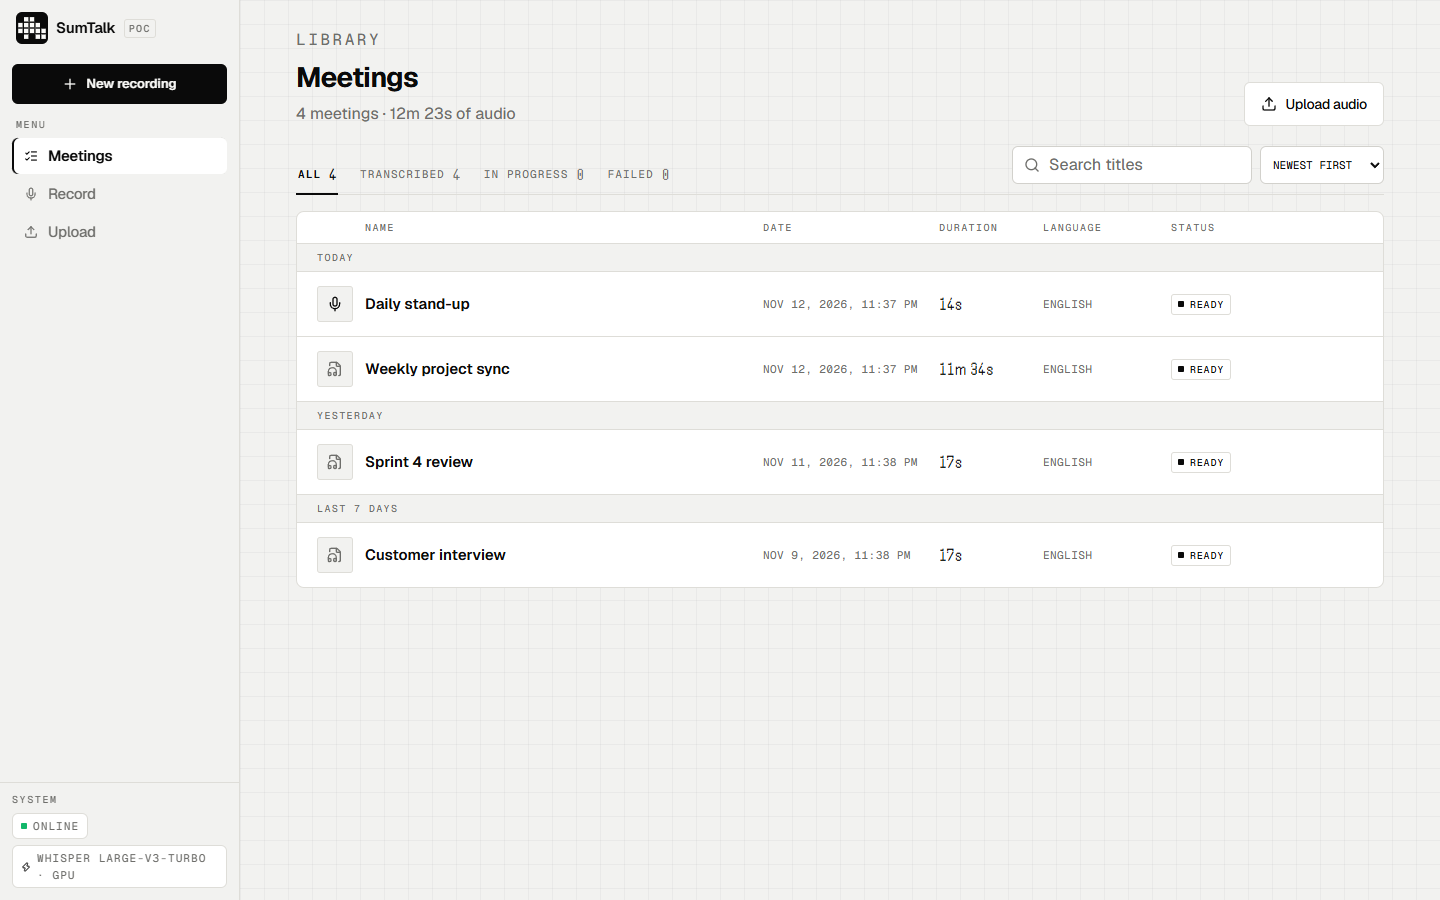
\includegraphics[width=0.82\linewidth]{meetings-list.png}}
  \caption{S1 -- Danh sách cuộc họp}
  \label{fig:meetings-list}
\end{figure}

\begin{table}[htbp]
  \centering
  \caption{S1 -- Thành phần và hành vi}
  \label{tab:s1}
  \small
  \begin{tabularx}{\linewidth}{@{}P{3cm}L@{}}
    \toprule
    \thead{Khu vực} & \thead{Thành phần và hành vi} \\
    \midrule
    Tiêu đề & Eyebrow \texttt{LIBRARY}, tiêu đề \ui{Meetings}, dòng tổng ``4 meetings · 12m 23s of audio''. Nút
      \ui{Upload audio}; trên điện thoại có thêm nút \ui{Record} \\
    Tab lọc & \ui{All / Transcribed / In progress / Failed}, kèm số lượng. Số \ui{Failed} chuyển đỏ khi $>$ 0. Tab
      \ui{In progress} hiện thêm dòng ``\textasciitilde Xm of transcription left'' \\
    Tìm kiếm & Ô \ui{Search titles} lọc theo tên khi đang gõ; có nút $\times$ để xoá \\
    Sắp xếp & \ui{Newest first / Oldest first / Longest first / Title A--Z}. Hai kiểu theo ngày thì nhóm thành
      \ui{Today / Yesterday / Last 7 days / Earlier} theo ngày lịch \\
    Bảng ($\geq$ 768\,px) & Cột \ui{Name, Date, Duration, Language, Status} và nút ⋯. Icon micro là bản ghi âm,
      icon file là bản upload. Bấm vào bất kỳ chỗ nào của dòng để mở cuộc họp \\
    Dòng (điện thoại) & Tên, rồi một dòng phụ gồm ngày · thời lượng · ngôn ngữ; badge trạng thái bên phải \\
    Menu ⋯ & \ui{Rename}: sửa tên ngay trên dòng (Enter lưu, Esc huỷ, bấm ra ngoài cũng lưu). \ui{Delete}: mở hộp
      thoại xác nhận (Mục~\ref{sec:dialogs}). Trên máy tính, nút ⋯ chỉ hiện khi rê chuột vào dòng \\
    Đang xử lý & Badge \ui{Transcribing 42\%} kèm ``\textasciitilde 3m left'' (ước lượng trên, giả định tốc độ
      bằng thời gian thực) \\
    Chờ upload & Khu \ui{Waiting to upload from this device} ở trên cùng, liệt kê bản ghi còn chunk trên máy, kèm
      số chunk và lỗi nếu có \\
    \bottomrule
  \end{tabularx}
\end{table}

Danh sách tự cập nhật mỗi 4 giây. Các trạng thái đặc biệt của màn hình được liệt kê trong Bảng~\ref{tab:s1-states};
trạng thái chưa có cuộc họp nào được minh hoạ ở Hình~\ref{fig:meetings-empty}.

\begin{table}[htbp]
  \centering
  \caption{S1 -- Các trạng thái của danh sách}
  \label{tab:s1-states}
  \small
  \begin{tabularx}{\linewidth}{@{}P{4.2cm}L@{}}
    \toprule
    \thead{Trạng thái} & \thead{Hiển thị} \\
    \midrule
    Đang tải & 3 dòng skeleton \\
    Chưa có cuộc họp & Icon hộp thư, ``No meetings yet'', hai nút \ui{New recording} và \ui{Upload audio} \\
    Lọc không ra kết quả & ``No meetings match'', nút \ui{Clear filters} \\
    Không gọi được server & Notice cảnh báo ``Can't load meetings from the server'', kèm lời nhắc bản ghi mới vẫn
      được giữ trên máy \\
    Đổi tên/xoá lỗi & Notice đỏ ``That didn't work'' \\
    \bottomrule
  \end{tabularx}
\end{table}

\begin{figure}[htbp]
  \centering
  \fbox{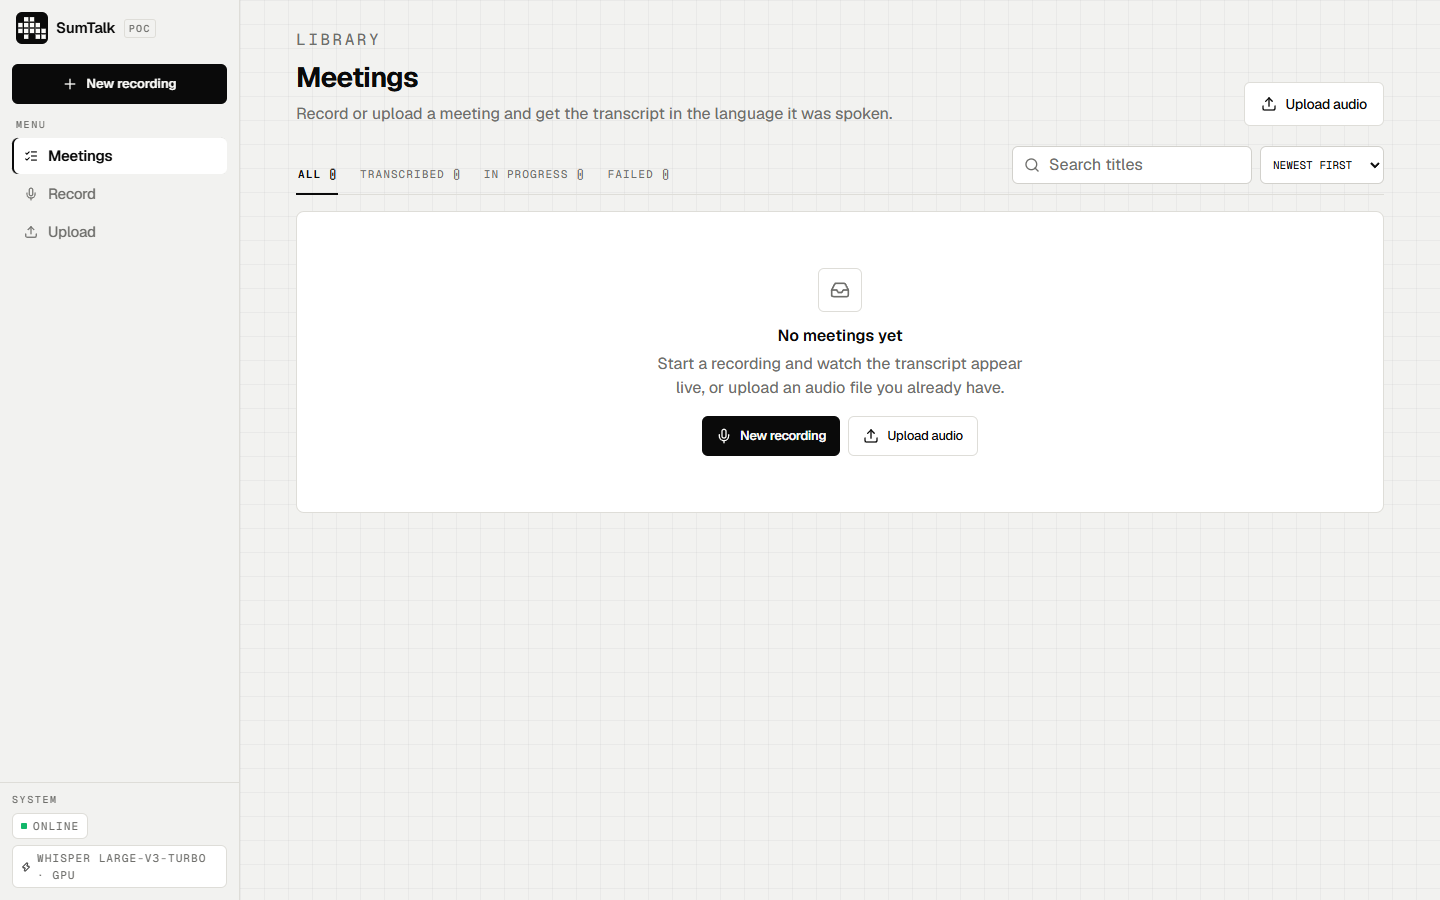
\includegraphics[width=0.82\linewidth]{meetings-empty.png}}
  \caption{S1 -- Trạng thái chưa có cuộc họp}
  \label{fig:meetings-empty}
\end{figure}

\section{S2 -- Ghi âm}

\textbf{Đường dẫn:} \texttt{/record}. \textbf{Mục đích:} ghi cuộc họp và xem transcript ngay khi nói.
\textbf{Story:} US1.1, US1.2, US2.2. Màn hình có hai trạng thái chính: trước khi ghi và đang ghi.

\subsection{Trước khi ghi}

Trước khi ghi, người dùng đặt tên, ngày, ngôn ngữ nói và nguồn âm thanh (Hình~\ref{fig:record-idle},
Bảng~\ref{tab:s2-idle}). Lỗi (trình duyệt không hỗ trợ, bị từ chối quyền micro) hiện thành Notice đỏ phía trên
form, có nút $\times$ để đóng.

\begin{figure}[htbp]
  \centering
  \fbox{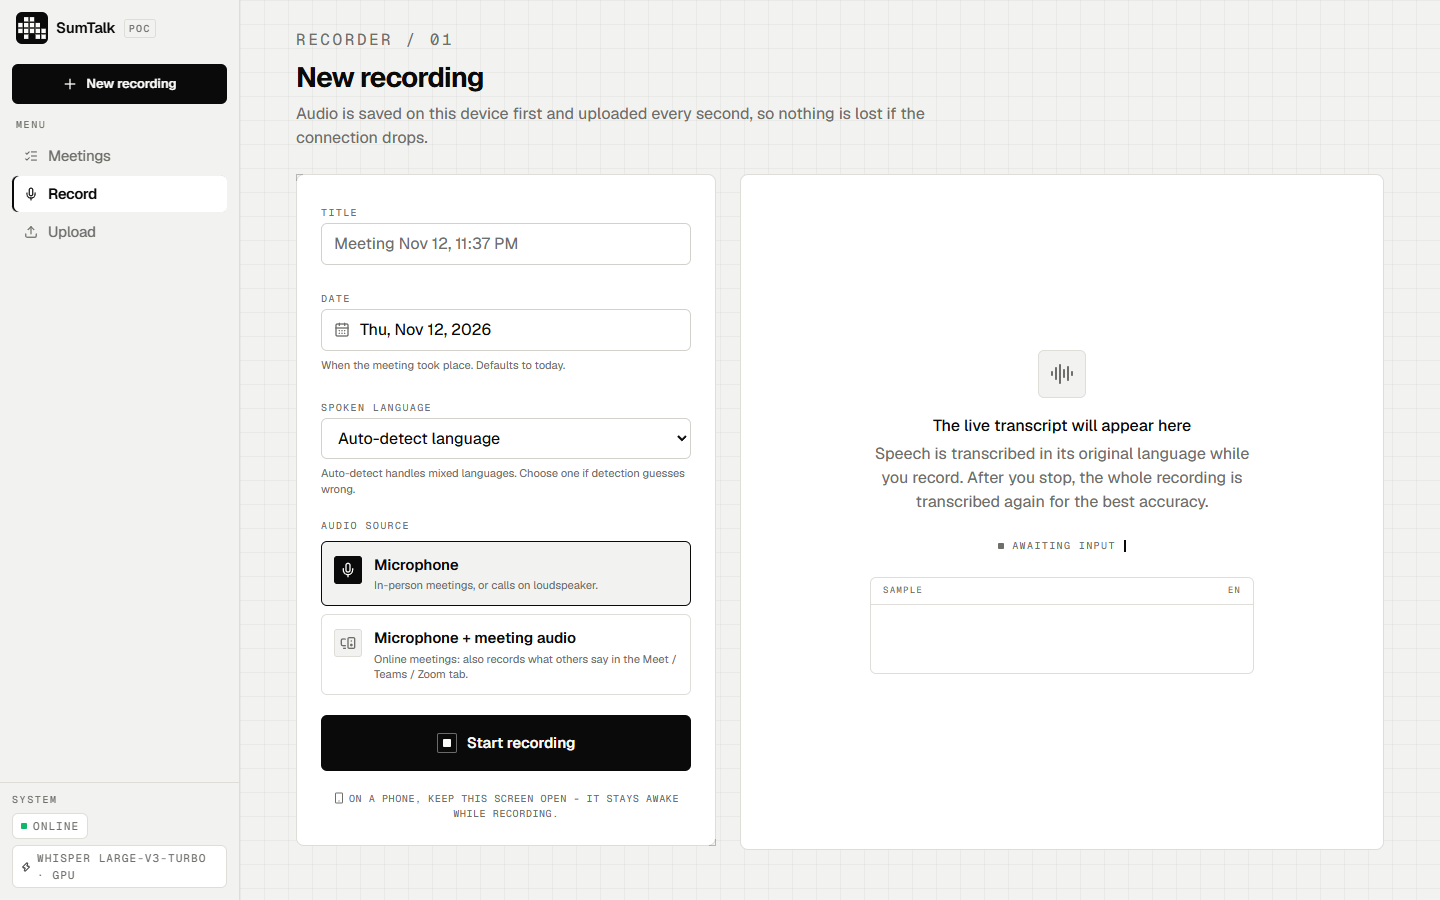
\includegraphics[width=0.82\linewidth]{record-idle.png}}
  \caption{S2 -- Màn ghi âm trước khi bắt đầu}
  \label{fig:record-idle}
\end{figure}

\begin{table}[htbp]
  \centering
  \caption{S2 -- Thành phần trước khi ghi}
  \label{tab:s2-idle}
  \small
  \begin{tabularx}{\linewidth}{@{}P{3.2cm}L@{}}
    \toprule
    \thead{Thành phần} & \thead{Hành vi} \\
    \midrule
    \ui{Title} & Để trống thì dùng tên mặc định ``Meeting <ngày giờ>'' (hiện sẵn ở placeholder) \\
    \ui{Date} & Chọn ngày diễn ra cuộc họp; mặc định hôm nay \\
    \ui{Spoken language} & \ui{Auto-detect language} (mặc định, xử lý được họp trộn ngôn ngữ) hoặc 1 trong 15 ngôn
      ngữ. Lựa chọn được nhớ cho lần sau \\
    \ui{Audio source} & Hai thẻ chọn. \ui{Microphone}: họp trực tiếp. \ui{Microphone + meeting audio}: thu cả tiếng
      người khác trong Meet/Teams/Zoom; bị làm mờ nếu trình duyệt không hỗ trợ (``Needs desktop Chrome or Edge.'') \\
    Notice theo nguồn & Chọn micro + âm thanh họp trên trình duyệt: hướng dẫn chọn tab họp và bật \ui{Share tab
      audio}. Trên app desktop: nhắc đeo tai nghe để tiếng không bị thu hai lần \\
    \ui{Start recording} & Nút chính cao 56\,px; khi đang khởi động thì đổi thành ``Starting\ldots'' \\
    Khung bên phải & ``The live transcript will appear here'', trạng thái \texttt{AWAITING INPUT} có con trỏ nhấp
      nháy, và một khung chữ mẫu tự gõ để minh hoạ (tắt hiệu ứng khi hệ thống bật giảm chuyển động) \\
    \bottomrule
  \end{tabularx}
\end{table}

\subsection{Đang ghi}

Khi đang ghi, màn hình chia hai cột: bên trái là đồng hồ, mức âm và các nút điều khiển; bên phải là transcript
live (Hình~\ref{fig:record-live}, Bảng~\ref{tab:s2-live}).

\begin{figure}[htbp]
  \centering
  \fbox{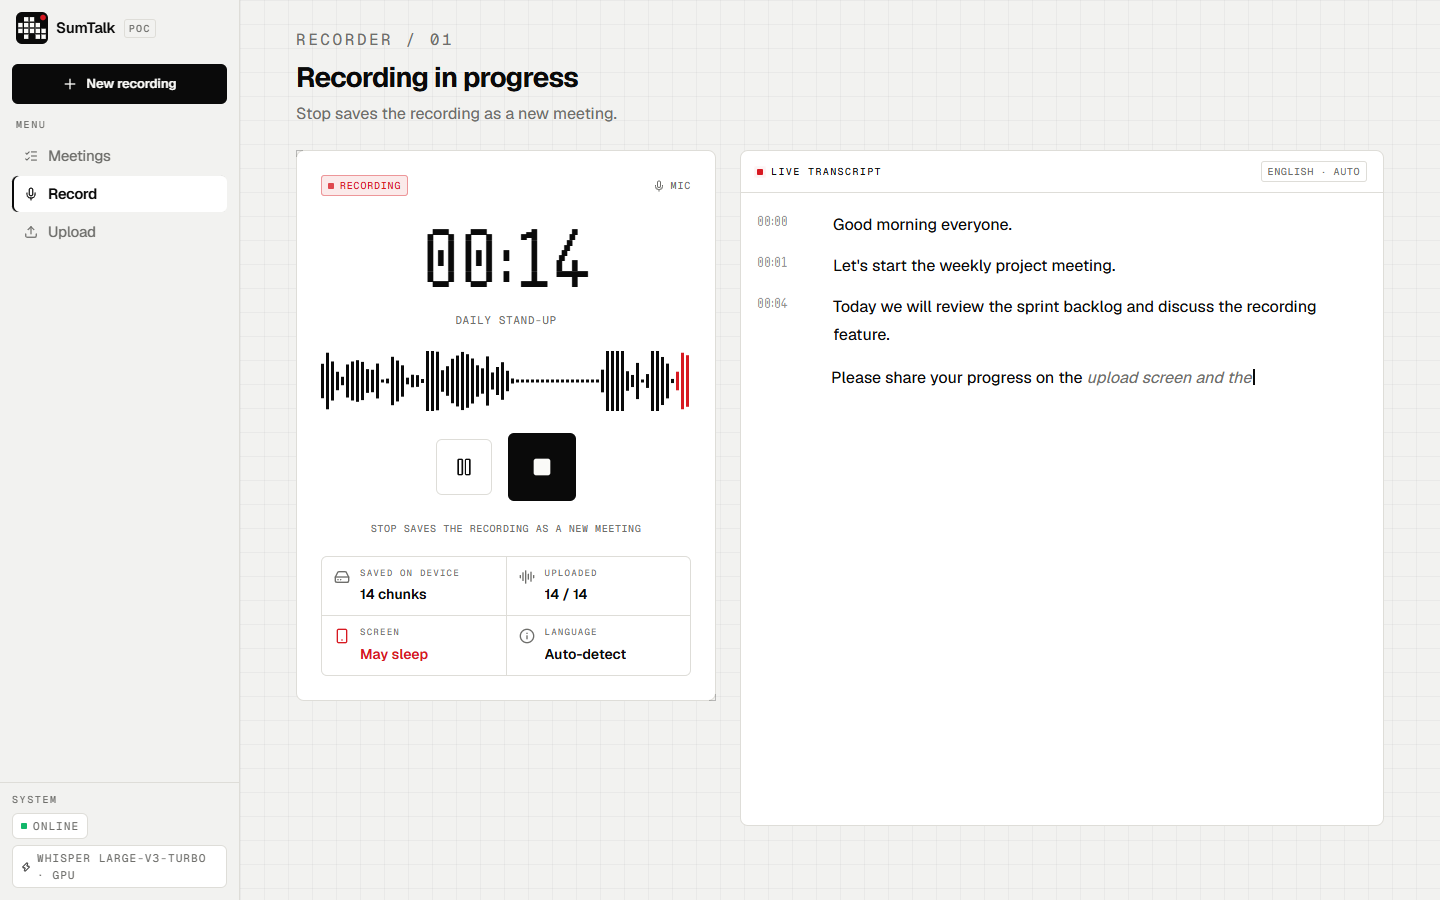
\includegraphics[width=0.82\linewidth]{record-live.png}}
  \caption{S2 -- Đang ghi, transcript hiện trực tiếp}
  \label{fig:record-live}
\end{figure}

\begin{table}[htbp]
  \centering
  \caption{S2 -- Thành phần khi đang ghi}
  \label{tab:s2-live}
  \small
  \begin{tabularx}{\linewidth}{@{}P{3.2cm}L@{}}
    \toprule
    \thead{Thành phần} & \thead{Hành vi} \\
    \midrule
    Badge trạng thái & \ui{Recording} (đỏ, nhấp nháy) / \ui{Paused} / \ui{Saving\ldots}; bên phải ghi nguồn đang
      thu (\ui{Mic} hoặc \ui{Mic + meeting audio}) \\
    Đồng hồ & Font số LED cỡ lớn, bên dưới là tên cuộc họp \\
    Level meter & Các vạch theo âm lượng thật; vạch mới nhất màu đỏ \\
    Nút & \ui{Pause/Resume} (48--56\,px) và \ui{Stop} (64--68\,px, nền đen). Bấm Stop thì lưu và mở trang cuộc họp \\
    4 ô thông số & \ui{Saved on device} (số chunk), \ui{Uploaded} (đã gửi / tổng; mất mạng thì hiện ``Offline -
      later'' màu đỏ), \ui{Screen} (\ui{Kept awake} / \ui{Keep it on} / \ui{May sleep}), \ui{Language} \\
    Khung \ui{Live transcript} & Chấm đỏ nhấp nháy, chip ngôn ngữ (``English · auto''). Mỗi dòng có mốc thời gian.
      Dòng cuối đang nói: phần đã chốt in đen, phần còn có thể đổi in nghiêng xám, con trỏ nhấp nháy \\
    Tự cuộn & Luôn cuộn theo chữ mới, trừ khi người dùng đã cuộn lên để đọc (cách đáy hơn 80\,px) \\
    Mất mạng & Khung transcript báo ``You are offline. Audio keeps being saved on this device\ldots''; audio vẫn
      được ghi \\
    \bottomrule
  \end{tabularx}
\end{table}

Chunk 1 giây được gửi lên server ngay; trang hỏi transcript mỗi 0,7 giây. Chữ thường hiện khoảng 1 giây sau khi
nói, theo Test Summary Report~\cite{qtd}. Ảnh được chụp bằng trình duyệt tự động nên ô \ui{Screen} hiện
\ui{May sleep}; trên điện thoại hỗ trợ Wake Lock, ô này hiện \ui{Kept awake}.

\section{S3 -- Upload}

\textbf{Đường dẫn:} \texttt{/upload}. \textbf{Mục đích:} biến file ghi âm có sẵn thành một cuộc họp.
\textbf{Story:} US1.3, US2.4. Hình~\ref{fig:upload} cho thấy màn hình trước và sau khi chọn file;
Bảng~\ref{tab:s3} mô tả hành vi.

\begin{figure}[htbp]
  \centering
  \begin{minipage}[t]{0.485\linewidth}
    \centering
    \fbox{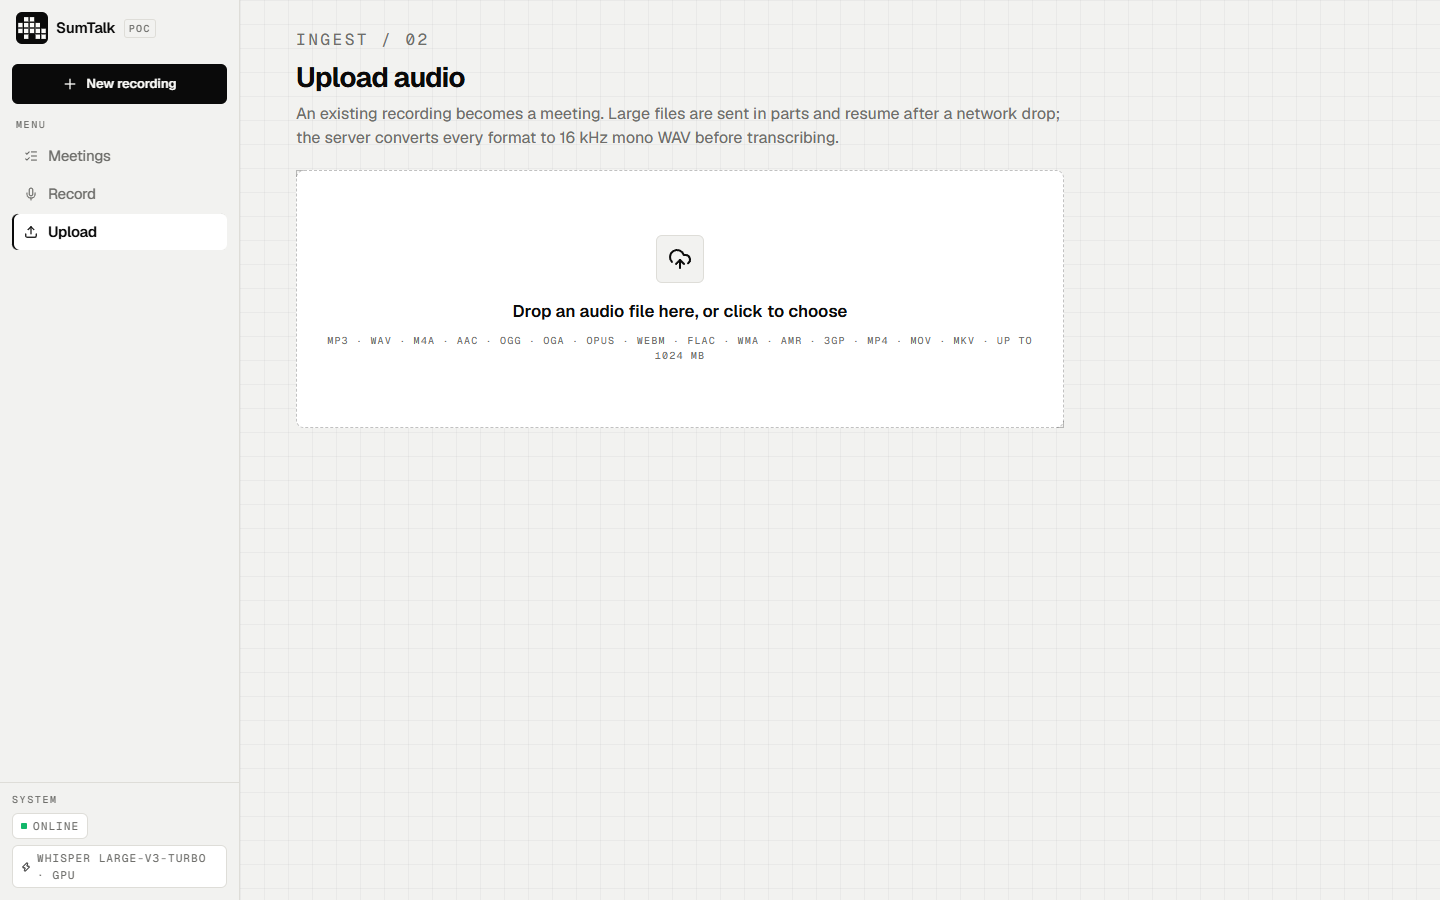
\includegraphics[width=0.96\linewidth]{upload-empty.png}}\\[2pt]
    {\footnotesize (a) Chưa chọn file}
  \end{minipage}\hfill
  \begin{minipage}[t]{0.485\linewidth}
    \centering
    \fbox{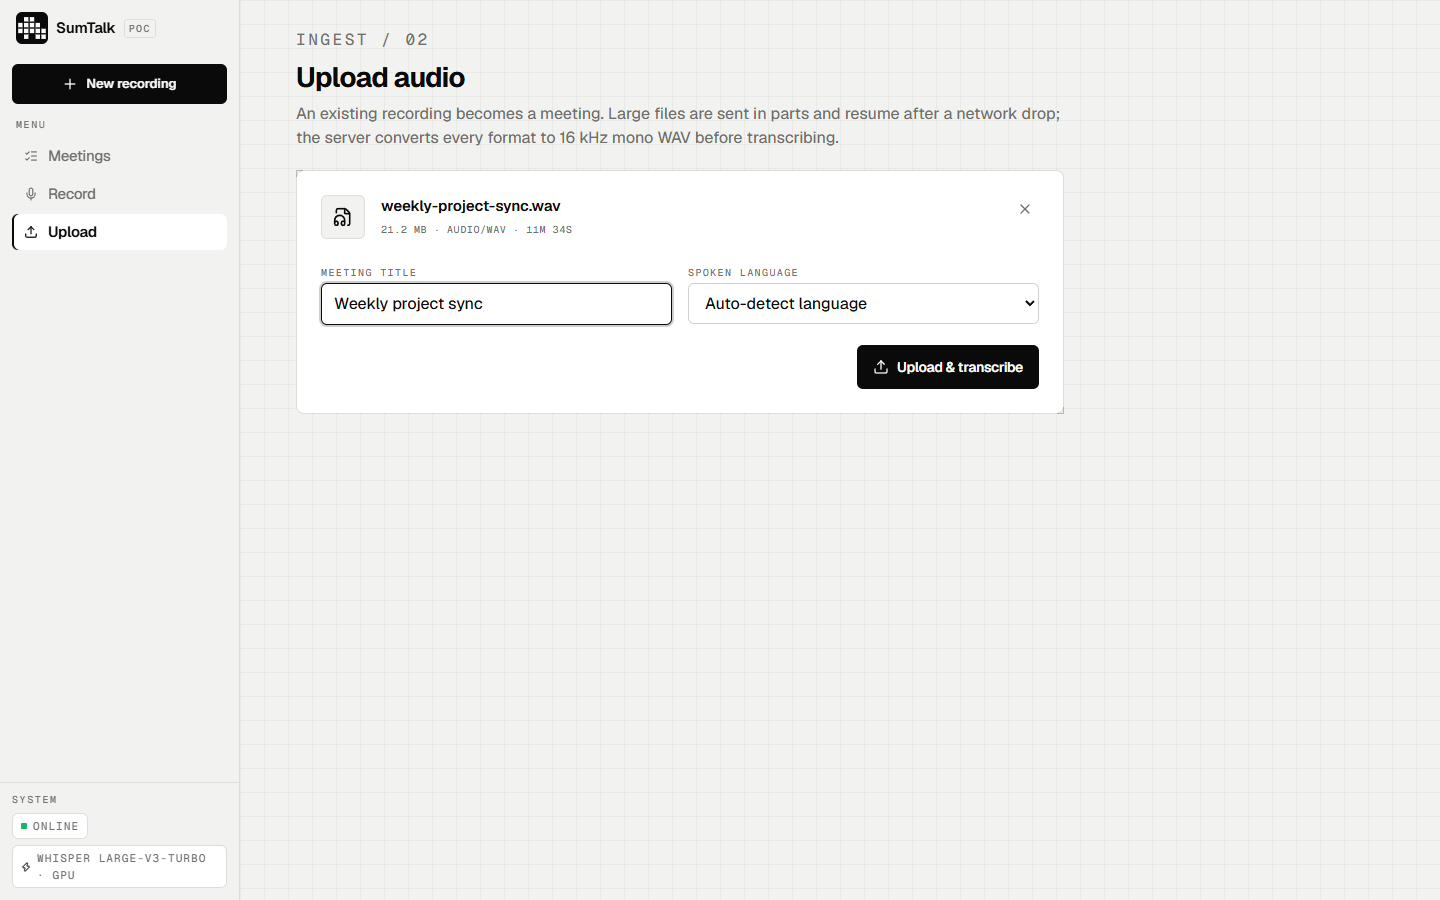
\includegraphics[width=0.96\linewidth]{upload-selected.png}}\\[2pt]
    {\footnotesize (b) Đã chọn file}
  \end{minipage}
  \caption{S3 -- Màn upload}
  \label{fig:upload}
\end{figure}

\begin{table}[htbp]
  \centering
  \caption{S3 -- Thành phần và hành vi}
  \label{tab:s3}
  \small
  \begin{tabularx}{\linewidth}{@{}P{3.4cm}L@{}}
    \toprule
    \thead{Thành phần} & \thead{Hành vi} \\
    \midrule
    Vùng thả file & Viền đứt, bấm để chọn hoặc kéo thả; khi kéo file vào thì viền đậm lên. Dòng dưới liệt kê
      định dạng hỗ trợ (MP3, WAV, M4A, AAC, OGG, OPUS, WEBM, FLAC, WMA, AMR, 3GP, MP4, MOV, MKV\ldots) và giới hạn
      ``up to 1024 MB'' \\
    Thẻ file & Tên file, dung lượng, loại, thời lượng (nếu trình duyệt đọc được); nút $\times$ để bỏ file \\
    Kiểm tra trước khi gửi & Báo lỗi ngay, không gửi: sai đuôi file, không phải audio/video, file rỗng, vượt dung
      lượng (``This file can't be used'') \\
    \ui{Meeting title} & Mặc định là tên file bỏ đuôi \\
    \ui{Spoken language} & Như màn ghi âm \\
    \ui{Upload \& transcribe} & Gửi theo từng phần, tự tiếp tục khi rớt mạng \\
    Khung tiến độ & Các bước \ui{Starting upload\ldots{} $\rightarrow$ Uploading\ldots{} $\rightarrow$ Creating the
      meeting\ldots}; khi mất mạng hiện \ui{Waiting for the network\ldots} với icon đỏ. Có \%, số byte, tốc độ,
      ``Part x / y'' và nút \ui{Cancel} \\
    Xong & Tự mở trang cuộc họp mới (S4) \\
    \bottomrule
  \end{tabularx}
\end{table}

\section{S4 -- Trang cuộc họp}

\textbf{Đường dẫn:} \texttt{/meetings/:id}. \textbf{Mục đích:} đọc, tìm, nghe lại, xuất transcript; xem tóm tắt
và bản dịch. \textbf{Story:} US2.1, US2.3, \#67, \#60. Đây là màn hình phức tạp nhất, gồm một khung chung và ba tab.

\subsection{Khung chung}

Khung chung gồm tiêu đề, dòng thông tin, khung trạng thái, ba tab và thanh phát audio (Hình~\ref{fig:meeting},
Bảng~\ref{tab:s4-frame}). Các hành động ít dùng được gom vào menu \ui{More actions} (Hình~\ref{fig:meeting-menu}).

\begin{figure}[htbp]
  \centering
  \fbox{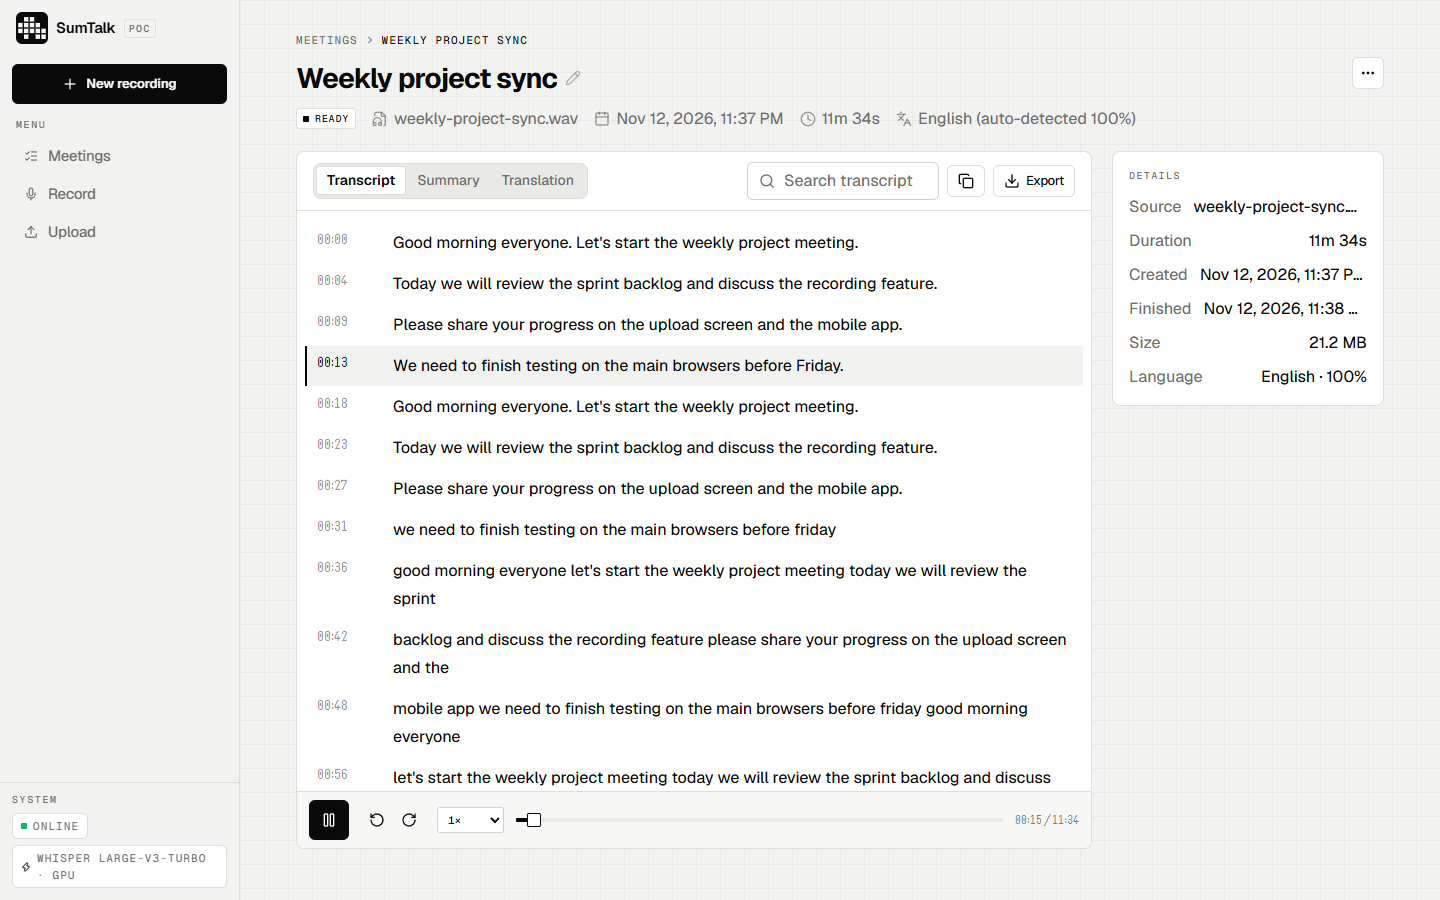
\includegraphics[width=0.82\linewidth]{meeting-transcript.png}}
  \caption{S4 -- Tab Transcript, đang phát audio}
  \label{fig:meeting}
\end{figure}

\begin{table}[htbp]
  \centering
  \caption{S4 -- Thành phần của khung chung}
  \label{tab:s4-frame}
  \small
  \begin{tabularx}{\linewidth}{@{}P{3.4cm}L@{}}
    \toprule
    \thead{Khu vực} & \thead{Thành phần và hành vi} \\
    \midrule
    Breadcrumb & Máy tính: \texttt{MEETINGS > TÊN CUỘC HỌP}. Điện thoại: \texttt{← MEETINGS} \\
    Tiêu đề & Bấm vào tên (có icon bút chì) để sửa; Enter hoặc bấm ra ngoài thì lưu, Esc thì huỷ \\
    Dòng thông tin & Badge trạng thái, nguồn (tên file / \ui{Microphone} / \ui{Mic + meeting audio}), ngày họp,
      thời lượng, ngôn ngữ (``English (auto-detected 100\%)''; họp trộn thì ``English + Vietnamese'') \\
    Menu ⋯ (\ui{More actions}) & \ui{Transcribe again\ldots} (làm mờ khi đang xử lý), \ui{Download audio (.wav)},
      \ui{Delete meeting} (đỏ) \\
    Khung trạng thái & Hiện giữa tiêu đề và nội dung, thay đổi theo trạng thái (Bảng~\ref{tab:s4-status}) \\
    Tab & \ui{Transcript} (có chữ đỏ \texttt{LIVE} khi đang là bản nháp live), \ui{Summary}, \ui{Translation} \\
    Thanh phát audio & Play/Pause, lùi/tới 10 giây, tốc độ 1$\times$ / 1,25$\times$ / 1,5$\times$ / 2$\times$,
      thanh tua, thời gian hiện tại / tổng \\
    Khung \ui{Details} ($\geq$ 1024\,px) & Source, Duration, Meeting, Created, Finished, Size, Chunks, Language
      (kèm độ tin cậy \%) \\
    \bottomrule
  \end{tabularx}
\end{table}

\begin{figure}[htbp]
  \centering
  \fbox{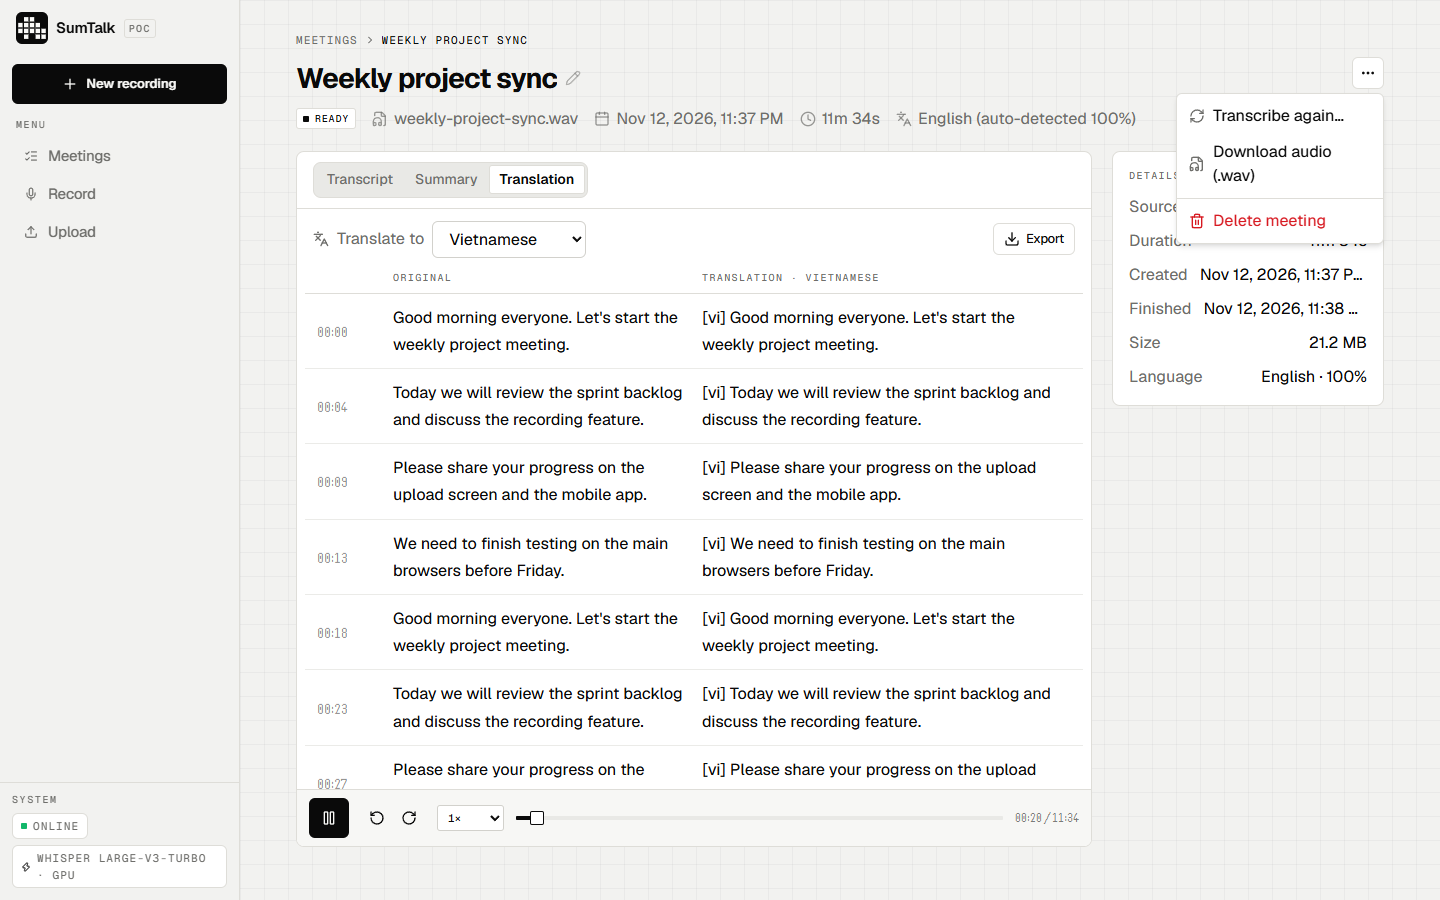
\includegraphics[width=0.82\linewidth]{meeting-menu.png}}
  \caption{S4 -- Menu More actions}
  \label{fig:meeting-menu}
\end{figure}

\subsection{Khung trạng thái theo tình huống}
\label{sec:s4-status}

Khung trạng thái cho người dùng biết cuộc họp đang ở bước nào và cần làm gì tiếp theo (Bảng~\ref{tab:s4-status}).

\begin{table}[htbp]
  \centering
  \caption{S4 -- Khung trạng thái theo tình huống}
  \label{tab:s4-status}
  \small
  \begin{tabularx}{\linewidth}{@{}P{4.6cm}L@{}}
    \toprule
    \thead{Tình huống} & \thead{Hiển thị} \\
    \midrule
    Đang ghi trên chính thiết bị này & ``Recording in progress'', link \ui{Open recorder} \\
    Đang upload chunk từ thiết bị này & ``Uploading the recording'', số chunk còn lại \\
    Đang ghi ở thiết bị/tab khác & ``Receiving audio'' \\
    Bị kẹt ở trạng thái ghi $>$ 20 giây & Cảnh báo ``Still marked as recording'', nút \ui{Finish now} để phiên âm
      phần đã nhận \\
    Upload file bị bỏ dở & ``Upload not finished'' \\
    Đang chờ / đang chuẩn hoá audio & ``Waiting in the queue\ldots'' / ``Converting audio to the standard
      format\ldots'', thanh chạy liên tục \\
    Đang phiên âm & ``Transcribing\ldots'' và \% (hoặc ``Loading the speech model\ldots''). Nếu đang hiện bản nháp
      live: ``Improving the transcript\ldots'' kèm ghi chú ``Showing the live draft until the accurate full-file
      transcript is ready.'' \\
    Lỗi & Notice đỏ ``Processing failed'', lý do, nút \ui{Retry} (nếu còn audio) \\
    \bottomrule
  \end{tabularx}
\end{table}

File dài được phiên âm theo từng đoạn khoảng 5 phút, nên các dòng hiện dần khi \% tăng
(Hình~\ref{fig:transcribing}); người dùng đọc được ngay mà không phải chờ hết file.

\begin{figure}[htbp]
  \centering
  \fbox{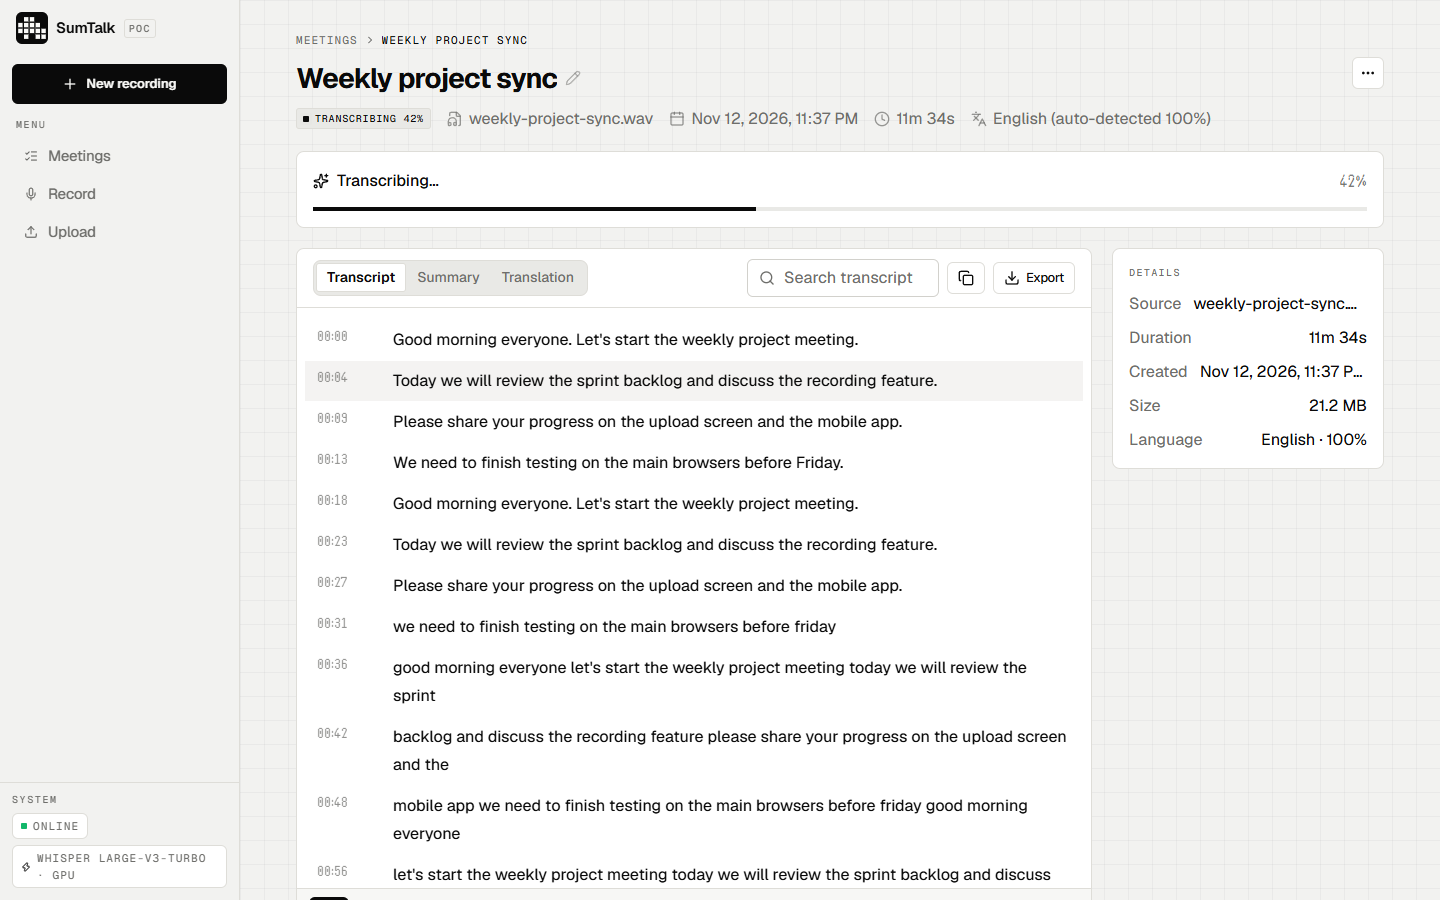
\includegraphics[width=0.82\linewidth]{meeting-transcribing.png}}
  \caption{S4 -- Đang phiên âm file dài, các dòng hiện dần}
  \label{fig:transcribing}
\end{figure}

\subsection{Tab Transcript}

Tab Transcript (Bảng~\ref{tab:s4-transcript}) là nơi đọc, tìm và nghe lại. Tìm kiếm chỉ giữ lại các dòng chứa từ
khoá (Hình~\ref{fig:search}).

\begin{table}[htbp]
  \centering
  \caption{S4 -- Tab Transcript}
  \label{tab:s4-transcript}
  \small
  \begin{tabularx}{\linewidth}{@{}P{3.4cm}L@{}}
    \toprule
    \thead{Thành phần} & \thead{Hành vi} \\
    \midrule
    Dòng transcript & Mốc thời gian (font LED) và nội dung. Bấm một dòng thì audio nhảy tới đó và phát \\
    Dòng đang phát & Nền xám và vạch đen bên trái; trang tự cuộn để dòng này luôn trong tầm nhìn \\
    Nhãn ngôn ngữ & Dòng nói khác ngôn ngữ chính có nhãn nhỏ bên phải (ví dụ \texttt{VI} trong cuộc họp tiếng Anh) \\
    \ui{Search transcript} & Chỉ giữ các dòng chứa từ khoá, tô nền từ khoá, hiện ``N lines match \ldots'' \\
    Nút copy & Chép toàn bộ transcript kèm mốc thời gian; icon đổi thành dấu ✓ trong 1,5 giây \\
    \ui{Export} & \ui{Text (.txt), Subtitles (.srt), WebVTT (.vtt), JSON (.json)} \\
    Trống & Đang xử lý: ``The transcript will appear here as soon as the first words are recognized.'' Xong mà
      không có lời nói: ``No speech was recognized in this audio.'' \\
    \bottomrule
  \end{tabularx}
\end{table}

\begin{figure}[htbp]
  \centering
  \fbox{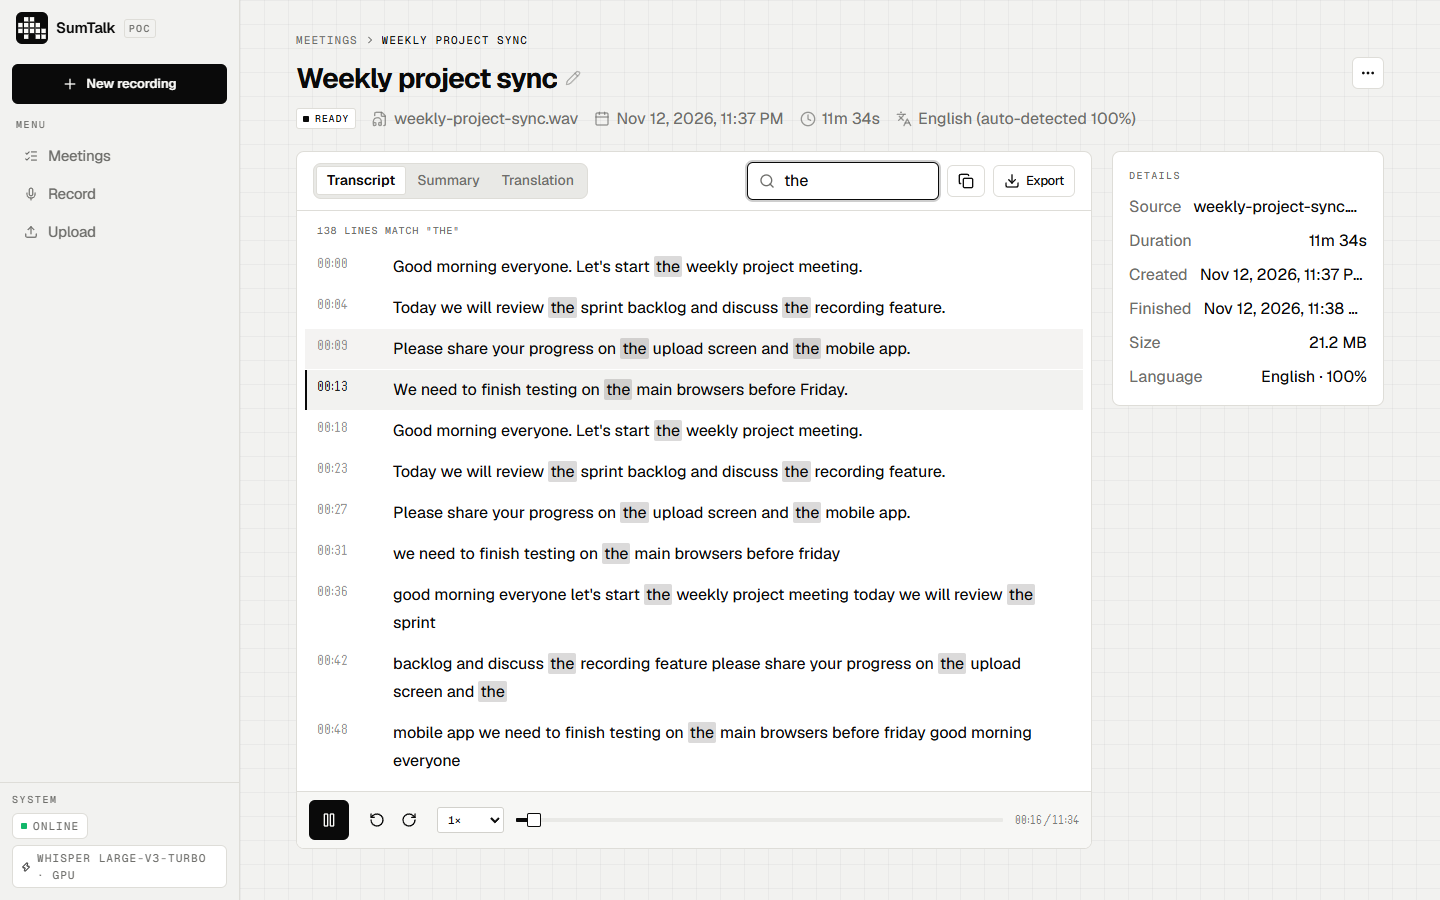
\includegraphics[width=0.82\linewidth]{meeting-search.png}}
  \caption{S4 -- Tìm trong transcript}
  \label{fig:search}
\end{figure}

\subsection{Tab Summary}

Tab Summary hiển thị biên bản do LLM tạo, chia thành năm phần (Hình~\ref{fig:summary}, Bảng~\ref{tab:s4-summary}).
Nội dung trong ảnh là chữ mẫu từ chế độ \texttt{AI\_MOCK}.

\begin{figure}[htbp]
  \centering
  \fbox{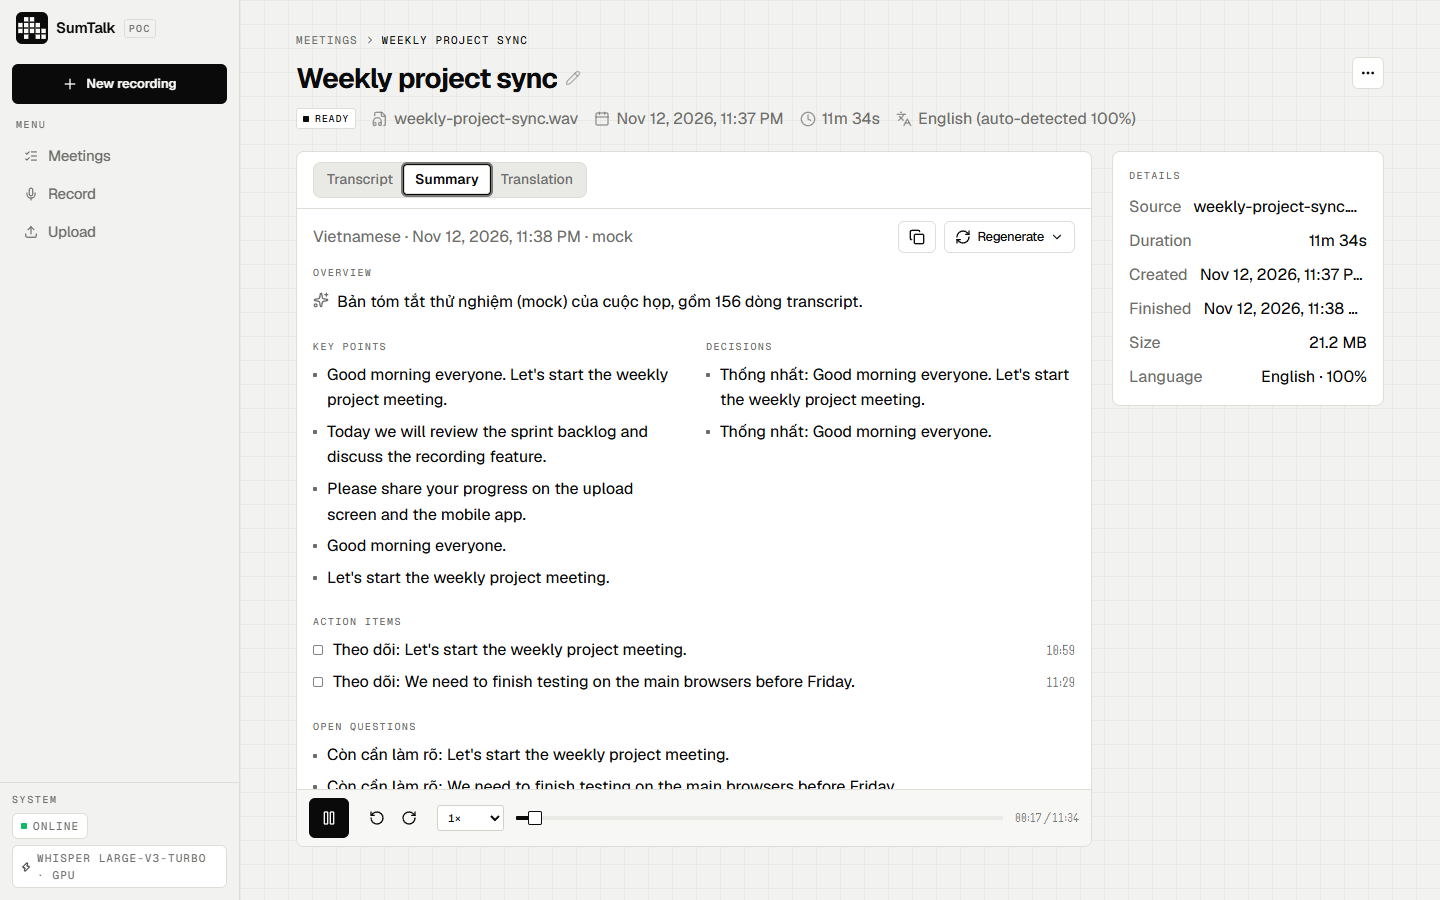
\includegraphics[width=0.82\linewidth]{meeting-summary.png}}
  \caption{S4 -- Tab Summary (nội dung mẫu từ AI\_MOCK)}
  \label{fig:summary}
\end{figure}

\begin{table}[htbp]
  \centering
  \caption{S4 -- Tab Summary: thành phần}
  \label{tab:s4-summary}
  \small
  \begin{tabularx}{\linewidth}{@{}P{4cm}L@{}}
    \toprule
    \thead{Thành phần} & \thead{Hành vi} \\
    \midrule
    Dòng thông tin & Ngôn ngữ · thời điểm tạo · model (ví dụ ``Vietnamese · Nov 12, 2026, 11:35 PM · mock'') \\
    Nút copy & Chép biên bản dạng chữ \\
    \ui{Regenerate ▾} (hoặc \ui{Generate}) & Chọn ngôn ngữ tóm tắt (Vietnamese / English); ngôn ngữ hiện tại có dấu
      ✓. Thay bản đã có thì phải xác nhận (Mục~\ref{sec:dialogs}) \\
    \ui{Overview} & Một đoạn tổng quan, có icon ✦ \\
    \ui{Key points} và \ui{Decisions} & Hai cột trên màn $\geq$ 768\,px, một cột trên điện thoại \\
    \ui{Action items} & Ô vuông, nội dung việc, người phụ trách · hạn (nếu có), mốc thời gian bấm được để nghe lại
      đoạn liên quan \\
    \ui{Open questions} & Danh sách câu hỏi còn mở \\
    \bottomrule
  \end{tabularx}
\end{table}

Tab Summary có năm trạng thái (Bảng~\ref{tab:s4-summary-states}); trong lúc đang tạo, trang hỏi lại kết quả mỗi
3 giây.

\begin{table}[htbp]
  \centering
  \caption{S4 -- Tab Summary: trạng thái}
  \label{tab:s4-summary-states}
  \small
  \begin{tabularx}{\linewidth}{@{}P{4cm}L@{}}
    \toprule
    \thead{Trạng thái} & \thead{Hiển thị} \\
    \midrule
    Transcript chưa xong & ``The summary is generated automatically as soon as the transcript is ready.'' \\
    Transcript lỗi & ``The transcript failed, so there is no summary.'' \\
    Chưa có tóm tắt & ``No summary yet. Use Generate to create one.'' \\
    Đang tạo & Vòng xoay, ``Summarizing\ldots'', ``Waiting for the summary model'' hoặc ``Writing the minutes in
      <ngôn ngữ>'', kèm ghi chú họp dài mất vài phút \\
    Lỗi & Notice đỏ ``The summary could not be generated'', nút \ui{Try again} \\
    \bottomrule
  \end{tabularx}
\end{table}

\subsection{Tab Translation}

Tab Translation hiển thị bản dịch song ngữ theo từng dòng (Hình~\ref{fig:translation}, Bảng~\ref{tab:s4-translation}).
Bản dịch được lưu lại, nên mở lại trang không phải dịch lại.

\begin{figure}[htbp]
  \centering
  \fbox{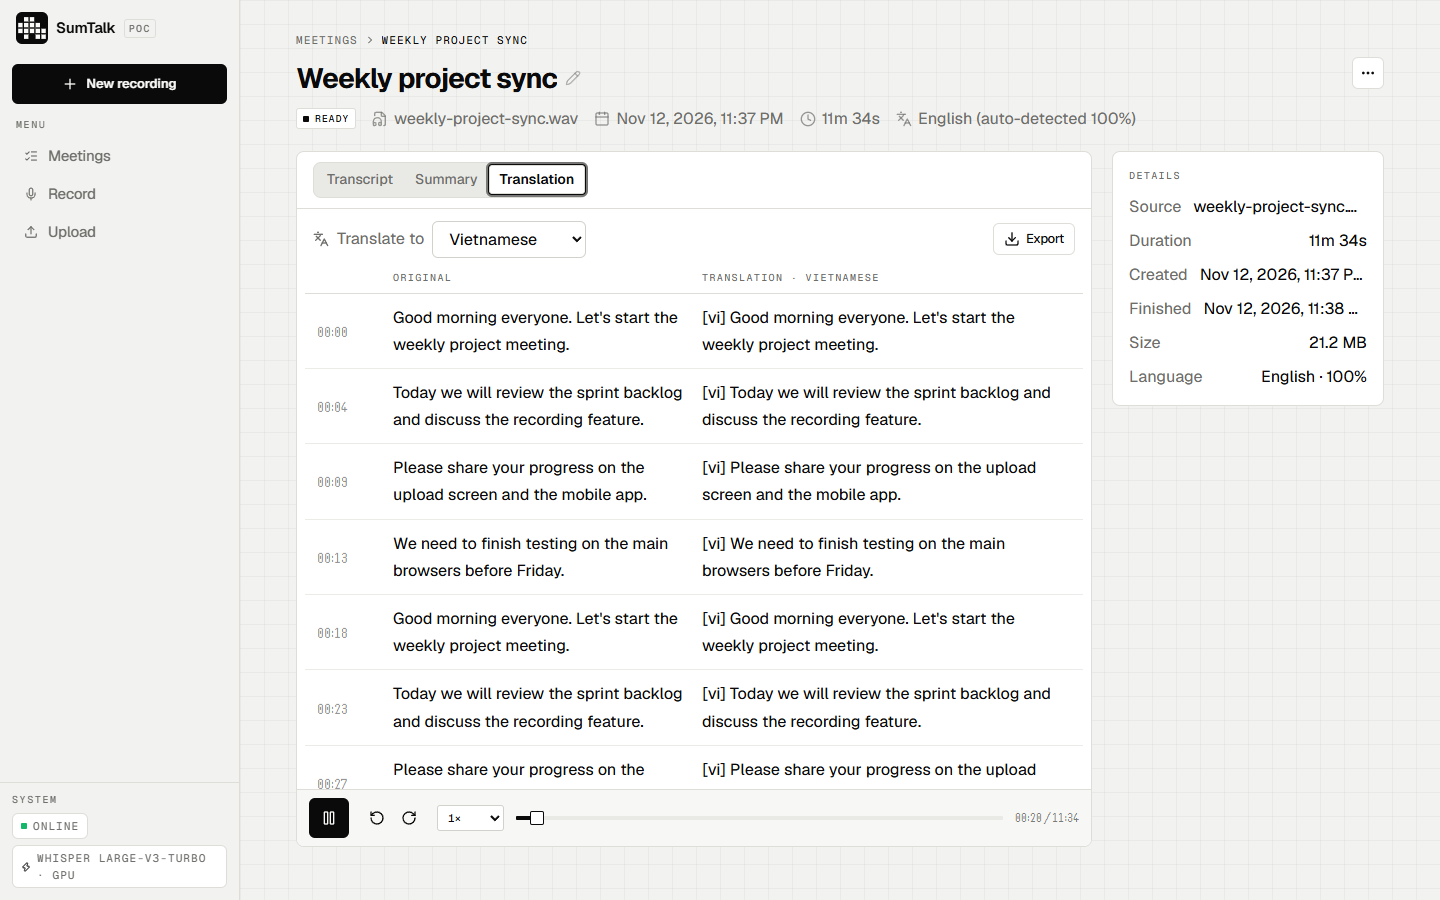
\includegraphics[width=0.82\linewidth]{meeting-translation.png}}
  \caption{S4 -- Tab Translation, hai cột (nội dung mẫu từ AI\_MOCK)}
  \label{fig:translation}
\end{figure}

\begin{table}[htbp]
  \centering
  \caption{S4 -- Tab Translation}
  \label{tab:s4-translation}
  \small
  \begin{tabularx}{\linewidth}{@{}P{3.8cm}L@{}}
    \toprule
    \thead{Thành phần} & \thead{Hành vi} \\
    \midrule
    \ui{Translate to} & Chọn Vietnamese / English; ngôn ngữ đã dịch xong có dấu ✓. Ngôn ngữ chọn lần trước được
      nhớ; mở lại trang thì hiện ngay bản đã lưu, không dịch lại \\
    Bảng hai cột & \ui{Original} \textbar{} \ui{Translation · Vietnamese}; mỗi dòng có mốc thời gian bấm được để nghe. Trên
      điện thoại, bản dịch nằm ngay dưới câu gốc \\
    Dòng chưa dịch & Thanh xám nhấp nháy (skeleton) \\
    Dòng vốn đã đúng ngôn ngữ đích & Giữ nguyên, có nhãn nhỏ ``already Vietnamese'' \\
    Tiến độ & ``Translating into Vietnamese\ldots{} 45\%'' và thanh tiến độ; hỏi lại mỗi 2 giây \\
    \ui{Export} (khi dịch xong) & \ui{Text (.txt)}, \ui{Subtitles (.srt)}, \ui{Text, original + translation},
      \ui{Subtitles, original + translation} \\
    Lỗi & Notice đỏ ``The translation stopped'', nút \ui{Try again}; các dòng đã dịch được giữ lại và có ghi số dòng \\
    Chưa chọn ngôn ngữ & ``Choose a language to translate the transcript. Lines already in that language are kept
      as they are.'' \\
    \bottomrule
  \end{tabularx}
\end{table}

\subsection{Cuộc họp chỉ có trên máy}

Khi mở một bản ghi chưa upload xong lên server (do mất mạng hoặc server tắt), trang cuộc họp hiển thị theo
Bảng~\ref{tab:s4-local}. Trạng thái này chưa có ảnh chụp.

\begin{table}[htbp]
  \centering
  \caption{S4 -- Cuộc họp chỉ có trên máy}
  \label{tab:s4-local}
  \small
  \begin{tabularx}{\linewidth}{@{}P{4.2cm}L@{}}
    \toprule
    \thead{Tình huống} & \thead{Hiển thị} \\
    \midrule
    Đang ghi trong tab/cửa sổ này & ``Recording in progress'' \\
    Có mạng, đang upload & ``Uploading from this device\ldots'', số chunk còn lại, phiên âm tự chạy sau đó \\
    Mất mạng & ``Saved on this device'', nhắc giữ trình duyệt và không xoá dữ liệu trình duyệt (app desktop: chunk
      được xử lý khi engine chạy lại) \\
    Server từ chối & Notice đỏ ``The server refused this recording'', nút \ui{Retry} và \ui{Discard} (cần xác nhận) \\
    Không tìm thấy & ``Meeting not found'', link \ui{Back to meetings} \\
    \bottomrule
  \end{tabularx}
\end{table}

\section{Trạng thái hệ thống}
\label{sec:system-status}

Khu \ui{System} trên sidebar (và thanh trên của điện thoại) có hai chip: kết nối và engine nhận dạng giọng nói.
Các trạng thái của chúng được liệt kê trong Bảng~\ref{tab:chips}.

\begin{table}[htbp]
  \centering
  \caption{Chip trạng thái hệ thống}
  \label{tab:chips}
  \small
  \begin{tabularx}{\linewidth}{@{}P{1.9cm}P{4.4cm}L@{}}
    \toprule
    \thead{Chip} & \thead{Trạng thái} & \thead{Hiển thị} \\
    \midrule
    Kết nối & Bình thường & Chấm xanh, \texttt{ONLINE} (trên điện thoại ẩn đi cho gọn) \\
            & Đang gửi chunk & Icon mây, \texttt{3 QUEUED} \\
            & Mất mạng / không gọi được server & Icon wifi gạch, chấm đỏ, \texttt{OFFLINE} hoặc \texttt{NO SERVER}
              kèm số chunk chờ; rê chuột thấy giải thích \\
    \midrule
    Engine  & Đang nạp model & Vòng xoay, \texttt{LOADING MODEL} \\
            & Sẵn sàng (chạy trên máy) & \texttt{WHISPER LARGE-V3-TURBO · GPU} (hoặc \texttt{· CPU}) \\
            & Sẵn sàng (engine remote) & Icon mây, \texttt{<model> · SERVER} \\
            & Lỗi model & Chữ đỏ, \texttt{SPEECH MODEL ERROR}; rê chuột thấy lý do \\
    \bottomrule
  \end{tabularx}
\end{table}

\section{Hộp thoại}
\label{sec:dialogs}

Ứng dụng có bốn hộp thoại (Bảng~\ref{tab:dialogs}; hai trong số đó được minh hoạ ở Hình~\ref{fig:dialogs}).
Hành động xoá luôn cần xác nhận và dùng màu đỏ. Esc hoặc \ui{Cancel} đóng hộp thoại mà không làm gì. Ba hộp
thoại xác nhận (Delete, Discard, Regenerate) không đóng khi bấm ra ngoài để tránh bấm nhầm; hộp thoại Transcribe
again thì có.

\begin{table}[htbp]
  \centering
  \caption{Các hộp thoại}
  \label{tab:dialogs}
  \small
  \begin{tabularx}{\linewidth}{@{}P{3.3cm}P{3.4cm}LP{2.4cm}@{}}
    \toprule
    \thead{Hộp thoại} & \thead{Khi nào} & \thead{Nội dung} & \thead{Nút} \\
    \midrule
    \ui{Delete this meeting?} & Delete từ danh sách hoặc từ trang cuộc họp & ``\textquotedbl<tên>\textquotedbl{} and its audio
      will be deleted. This cannot be undone.'' & \ui{Cancel}, \ui{Delete} (đỏ) \\
    \ui{Discard this recording?} & Discard bản ghi bị server từ chối & Xoá khỏi máy, không khôi phục được
      & \ui{Cancel}, \ui{Discard} (đỏ) \\
    \ui{Regenerate the summary?} & Chọn ngôn ngữ khi đã có tóm tắt & ``The current summary will be replaced by a new
      one in <ngôn ngữ>.'' & \ui{Cancel}, \ui{Regenerate} \\
    \ui{Transcribe again} & Menu ⋯ $\rightarrow$ Transcribe again\ldots & Chọn lại ngôn ngữ nói khi nhận sai;
      transcript cũ bị thay & \ui{Cancel}, \ui{Start} \\
    \bottomrule
  \end{tabularx}
\end{table}

\begin{figure}[htbp]
  \centering
  \begin{minipage}[t]{0.485\linewidth}
    \centering
    \fbox{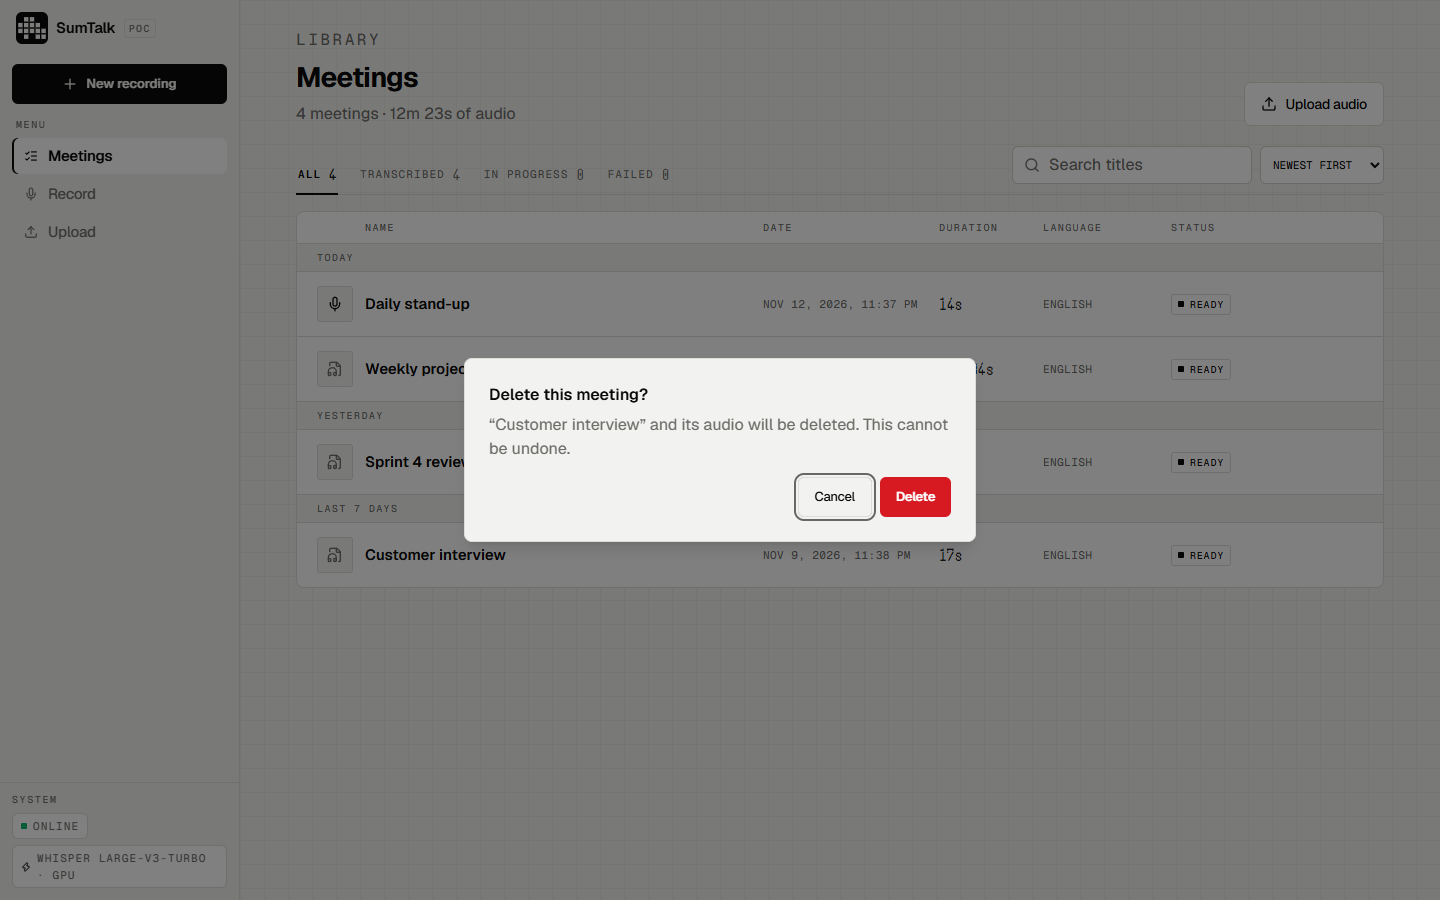
\includegraphics[width=0.96\linewidth]{dialog-delete.png}}\\[2pt]
    {\footnotesize (a) Xoá cuộc họp}
  \end{minipage}\hfill
  \begin{minipage}[t]{0.485\linewidth}
    \centering
    \fbox{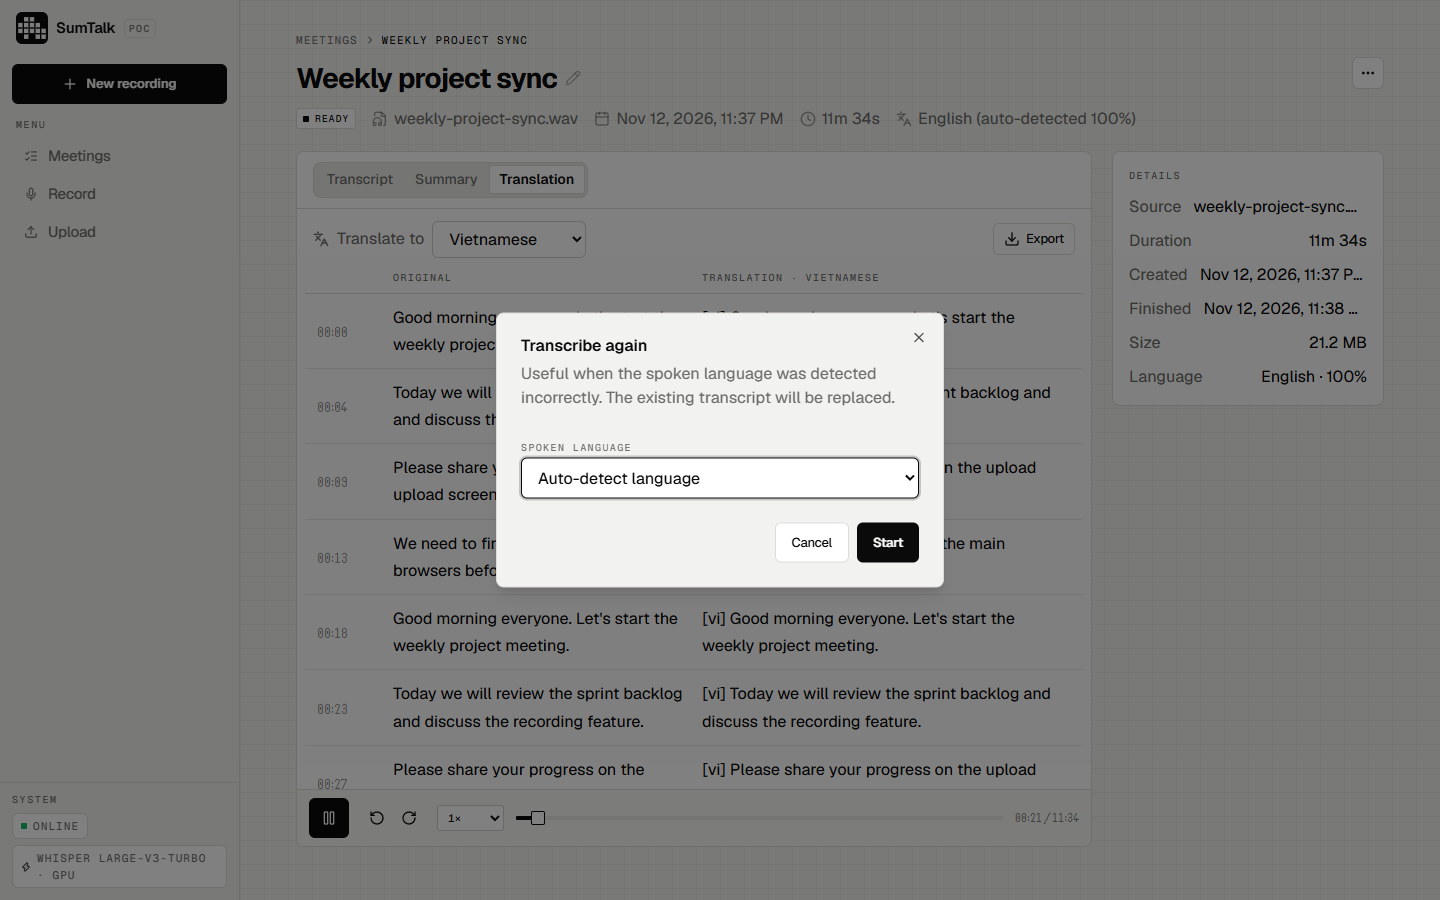
\includegraphics[width=0.96\linewidth]{dialog-retranscribe.png}}\\[2pt]
    {\footnotesize (b) Phiên âm lại}
  \end{minipage}
  \caption{Hộp thoại xoá cuộc họp và phiên âm lại}
  \label{fig:dialogs}
\end{figure}

\section{Điện thoại và app desktop}

\subsection{Điện thoại}

Trên điện thoại (390$\times$844), giao diện chuyển sang một cột với thanh menu dưới (Hình~\ref{fig:mobile}). Ảnh
``Đang ghi'' được chụp trên màn hình cao 1400\,px để thấy cả đồng hồ lẫn transcript; trên điện thoại thật, người
dùng cuộn xuống để xem transcript.

\begin{figure}[htbp]
  \centering
  \begin{minipage}[b]{0.27\linewidth}
    \centering
    \fbox{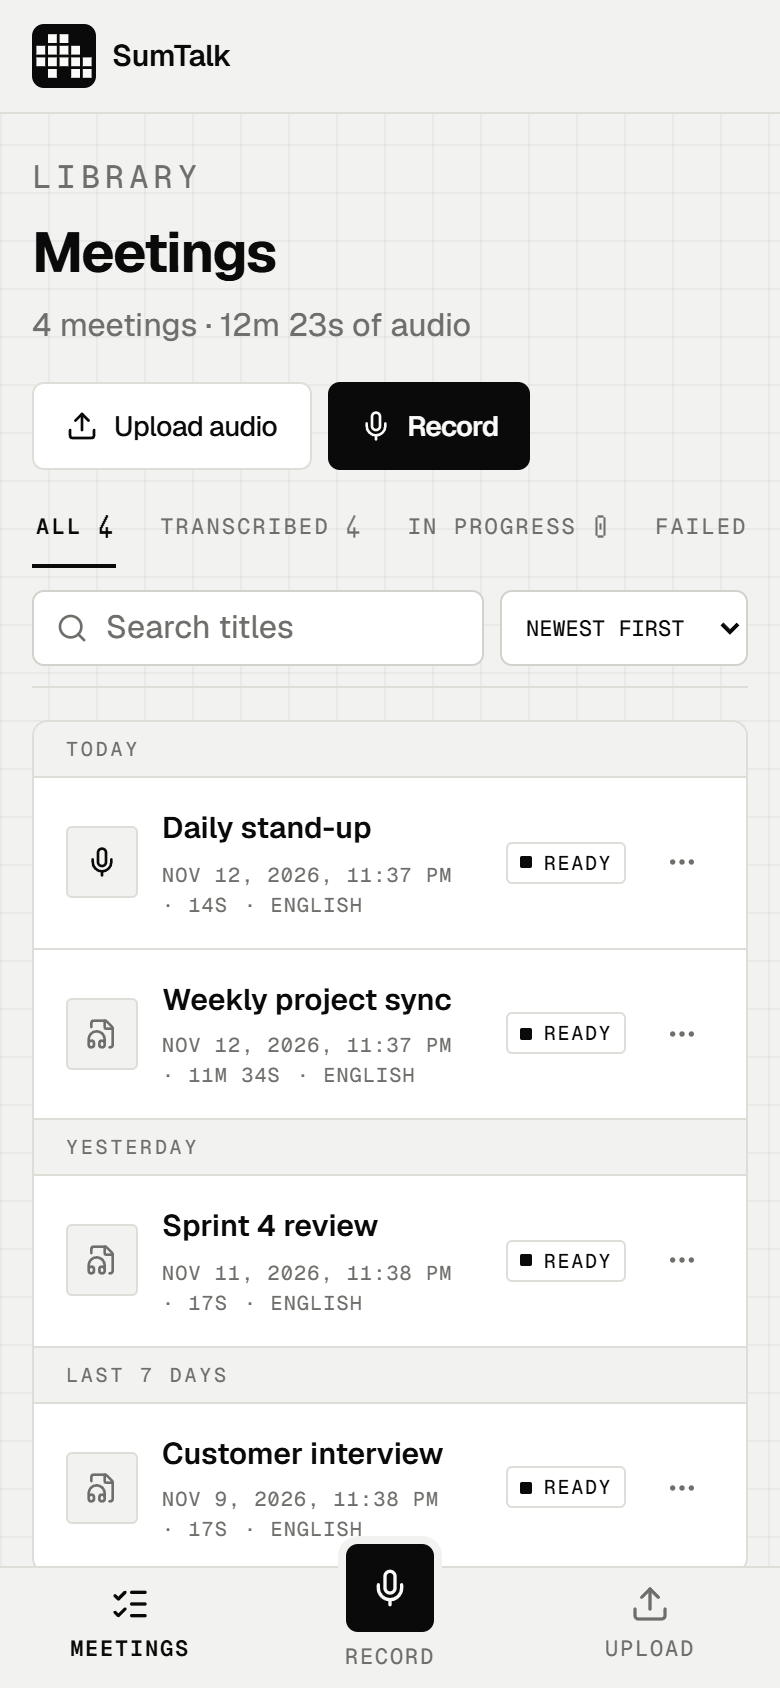
\includegraphics[height=8.2cm]{mobile-meetings.png}}\\[2pt]
    {\footnotesize (a) Danh sách}
  \end{minipage}\hfill
  \begin{minipage}[b]{0.27\linewidth}
    \centering
    \fbox{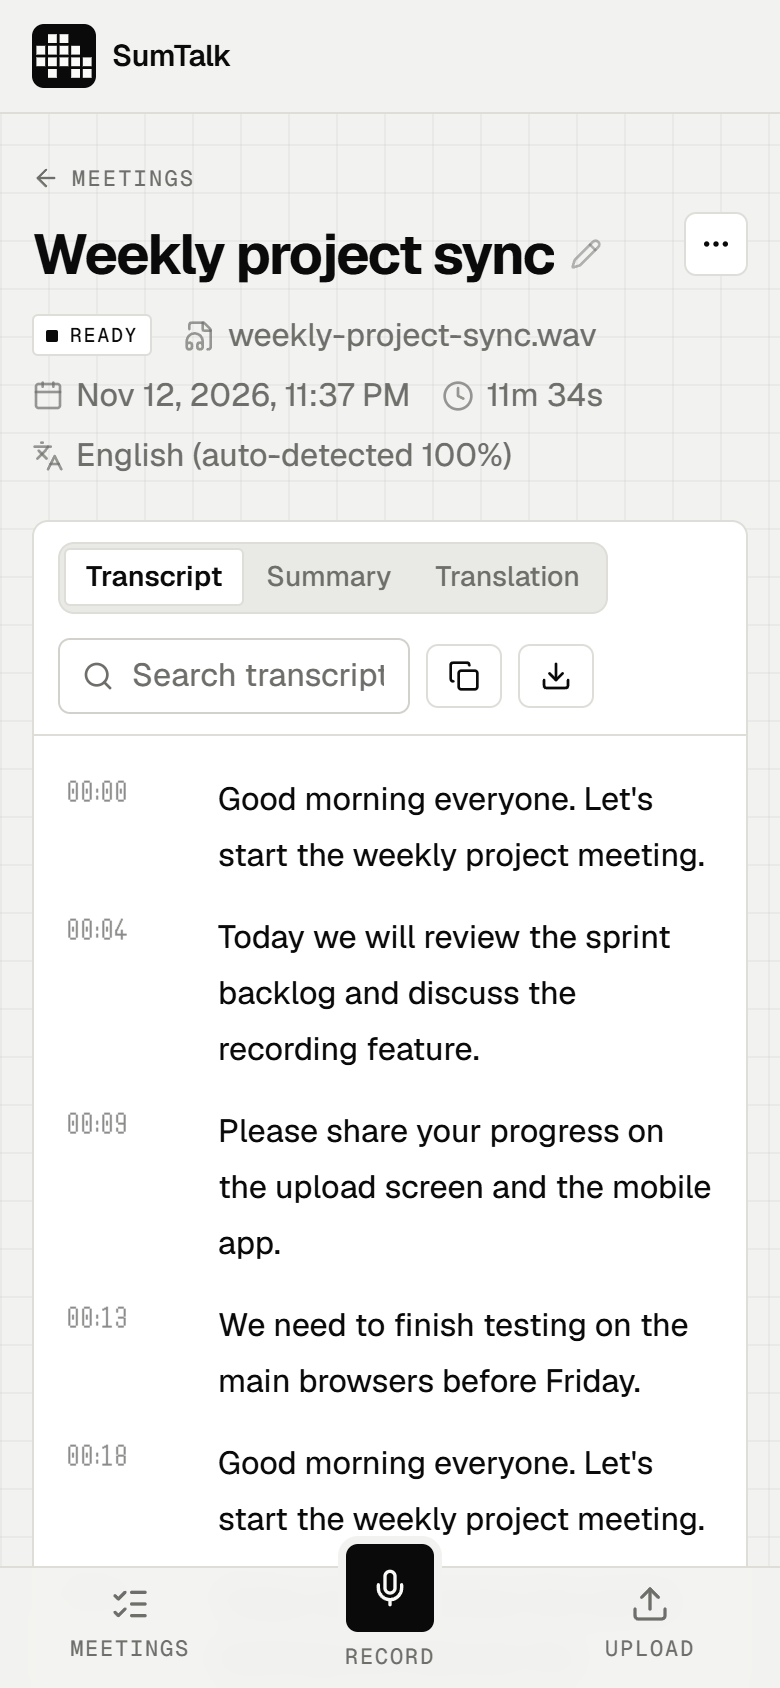
\includegraphics[height=8.2cm]{mobile-meeting.png}}\\[2pt]
    {\footnotesize (b) Trang cuộc họp}
  \end{minipage}\hfill
  \begin{minipage}[b]{0.27\linewidth}
    \centering
    \fbox{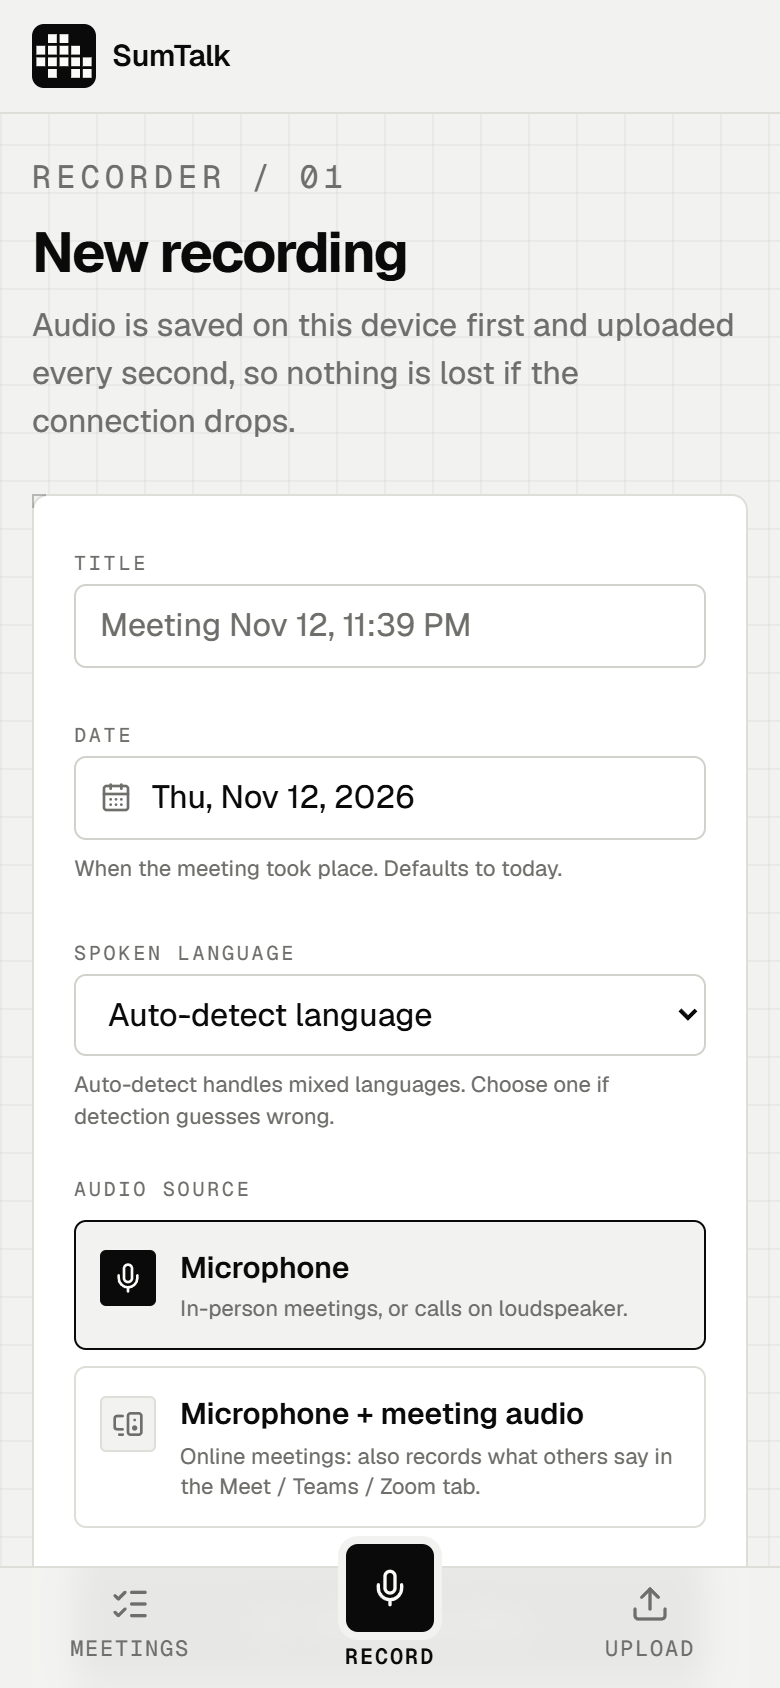
\includegraphics[height=8.2cm]{mobile-record-idle.png}}\\[2pt]
    {\footnotesize (c) Trước khi ghi}
  \end{minipage}\hfill
  \begin{minipage}[b]{0.17\linewidth}
    \centering
    \fbox{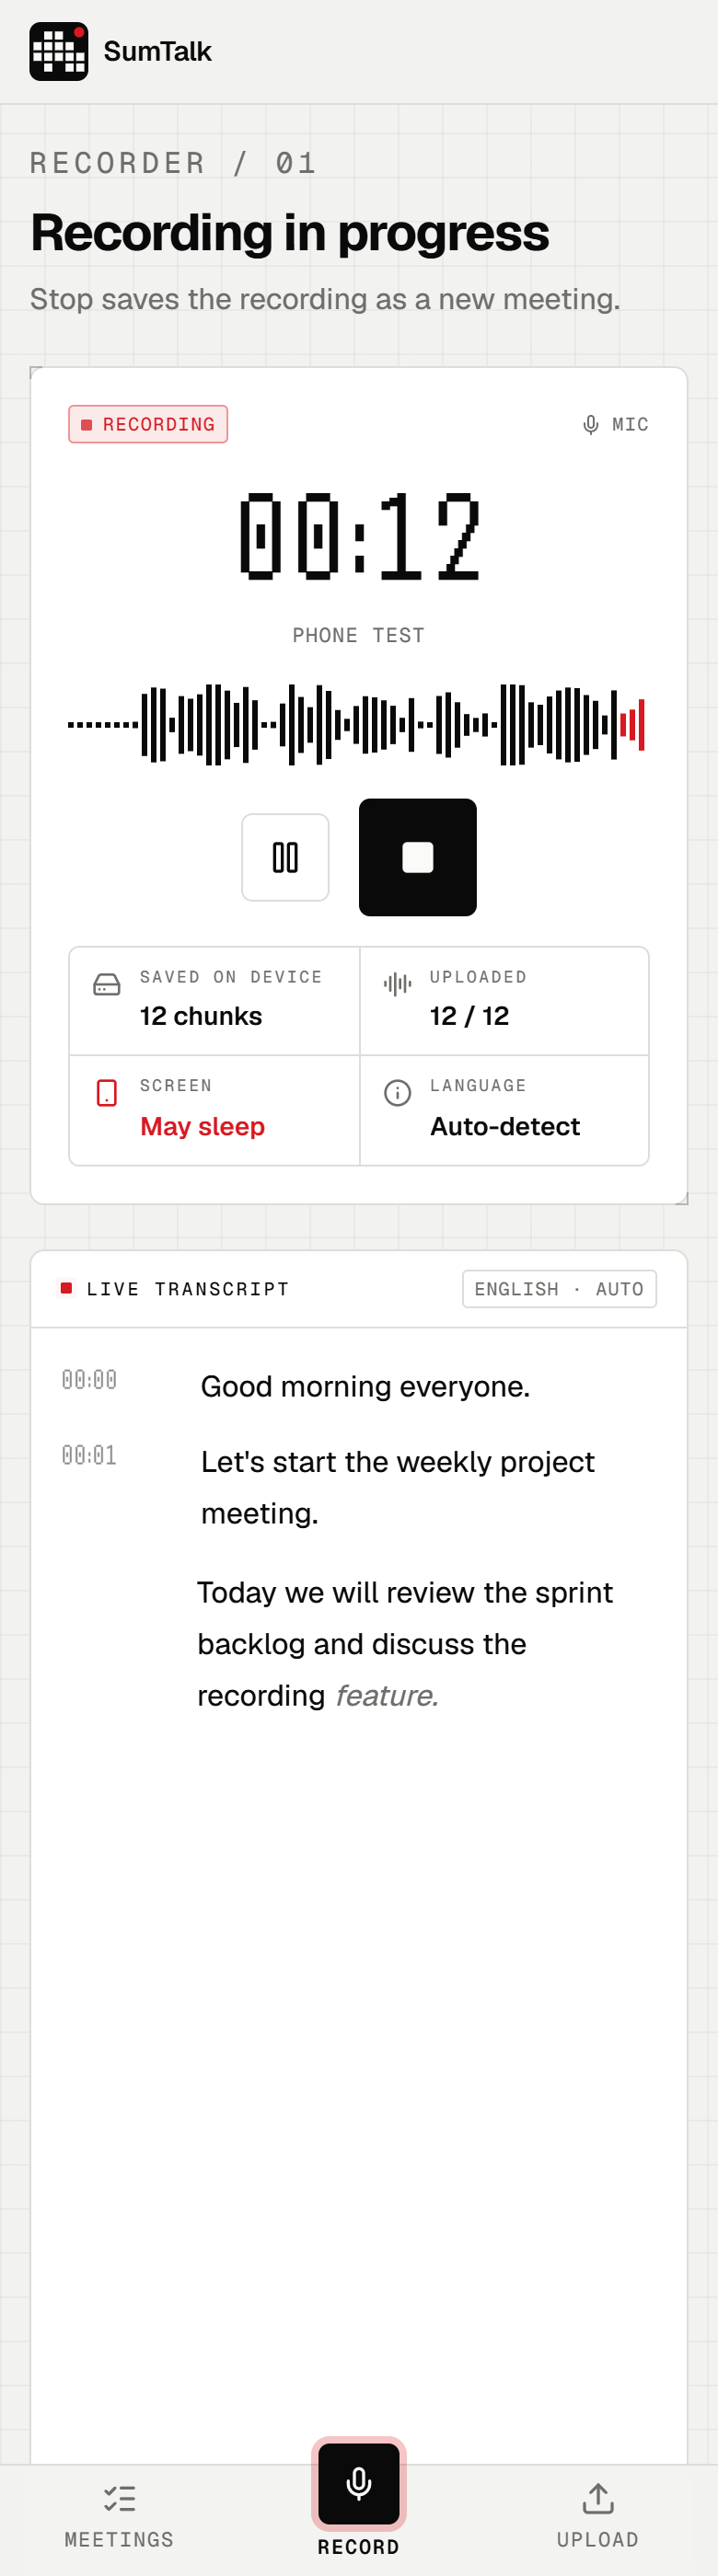
\includegraphics[height=8.2cm]{mobile-record-live.png}}\\[2pt]
    {\footnotesize (d) Đang ghi}
  \end{minipage}
  \caption{Giao diện trên điện thoại}
  \label{fig:mobile}
\end{figure}

\begin{itemize}
  \item \textbf{Thanh menu dưới:} 3 mục; nút \ui{Record} nổi lên, có viền đỏ nhạt khi đang ghi.
  \item \textbf{Danh sách:} bảng cuộc họp gộp thành một dòng phụ; nút ⋯ luôn hiện (không có hover).
  \item \textbf{Trang cuộc họp:} nút \ui{Export} chỉ còn icon; khung Details ẩn (thông tin chính đã có ở dòng dưới
        tiêu đề).
  \item \textbf{Khi ghi:} màn hình được giữ sáng (Wake Lock). iOS vẫn dừng micro khi khoá màn hình, đây là giới hạn
        của trình duyệt (rủi ro R13 trong~\cite{pmp}).
\end{itemize}

\subsection{App desktop}

App Windows (Electron) dùng cùng giao diện web, chỉ khác ở bốn điểm:
\begin{itemize}
  \item \textbf{Khởi động:} màn chờ ``SumTalk -- Starting\ldots'' trong lúc engine khởi động (khoảng 1,4--1,9 giây).
  \item \textbf{Nguồn âm thanh:} \ui{Microphone + meeting audio} thu toàn bộ âm thanh máy đang phát (Zoom/Teams/Meet
        bản desktop), không cần chọn tab. Mô tả và Notice nhắc đeo tai nghe để tiếng không bị thu hai lần.
  \item \textbf{Câu chữ:} ``this browser'' đổi thành ``this window'' / ``this computer''; bản ghi chưa xử lý được nói
        là sẽ chạy khi ``SumTalk engine'' hoạt động lại.
  \item \textbf{Engine remote:} khi dùng \texttt{STT\_PROVIDER=remote}, chip engine hiện \texttt{· SERVER} thay vì
        \texttt{GPU}/\texttt{CPU}.
\end{itemize}

\section{Khả năng truy cập và chu kỳ cập nhật dữ liệu}

\heading{Khả năng truy cập}
\begin{itemize}
  \item Nút chỉ có icon đều có \texttt{aria-label} (ví dụ ``Stop and save'', ``Copy transcript'', ``Actions for
        <tên>'').
  \item Có viền focus rõ khi dùng bàn phím (\texttt{focus-visible}).
  \item Sửa tên dùng Enter/Esc; hộp thoại đóng bằng Esc.
  \item Tôn trọng cài đặt giảm chuyển động của hệ thống (\texttt{prefers-reduced-motion}).
  \item Thông báo đang chạy (tóm tắt, dịch) dùng \texttt{role="status"}.
\end{itemize}

\heading{Chu kỳ cập nhật dữ liệu (polling)}
Giao diện lấy dữ liệu mới bằng cách hỏi server định kỳ; chu kỳ ngắn nhất dành cho transcript khi đang ghi, để giữ
độ trễ hiển thị khoảng 1\,s (Bảng~\ref{tab:polling}).

\begin{table}[htbp]
  \centering
  \caption{Chu kỳ cập nhật dữ liệu}
  \label{tab:polling}
  \begin{tabularx}{0.75\linewidth}{@{}Lr@{}}
    \toprule
    \thead{Nơi} & \thead{Chu kỳ} \\
    \midrule
    Transcript khi đang ghi & 0,7 giây \\
    Trang cuộc họp khi đang xử lý & 1,5 giây \\
    Danh sách cuộc họp & 4 giây \\
    Tab Summary khi đang tạo & 3 giây \\
    Tab Translation khi đang dịch & 2 giây \\
    \bottomrule
  \end{tabularx}
\end{table}

\section{Hạn chế và đề xuất cải tiến UI/UX}
\label{sec:ux-improve}

Tám hạn chế của giao diện hiện tại được liệt kê trong Bảng~\ref{tab:ux-improve}. Năm hạn chế gắn với story đã có
trong backlog tương lai (Bảng~\ref{tab:future}); ba hạn chế còn lại (UX-01, UX-02, UX-08) là đề xuất mới, cần PO
xem xét đưa vào backlog.

% Last table of the chapter: [H] so it is not pushed onto a page of its own.
\begin{table}[H]
  \centering
  \caption{Hạn chế và đề xuất cải tiến UI/UX}
  \label{tab:ux-improve}
  \small
  \begin{tabularx}{\linewidth}{@{}P{1.3cm}LLP{2.2cm}@{}}
    \toprule
    \thead{\#} & \thead{Hạn chế hiện tại} & \thead{Đề xuất} & \thead{Liên quan} \\
    \midrule
    UX-01 & Chữ giao diện chỉ có tiếng Anh, trong khi người dùng chính nói tiếng Việt & Thêm bản tiếng Việt cho giao
      diện (i18n), chọn theo ngôn ngữ trình duyệt & Đề xuất mới \\
    UX-02 & Chưa có dark mode & Thêm bộ token tối theo \texttt{prefers-color-scheme} & Đề xuất mới \\
    UX-03 & Không có tên người nói trên transcript & Nhận diện người nói, hiện ``Người nói:'' ở đầu dòng & US8.1 \\
    UX-04 & Việc cần làm chỉ nằm trong tab Summary & Trang action items riêng, liên kết tới đoạn transcript & \#79 \\
    UX-05 & Bản dịch chỉ có sau khi họp xong & Dịch trực tiếp trong khung live transcript & \#84 \\
    UX-06 & iOS dừng ghi khi khoá màn hình & App native, hoặc cảnh báo rõ hơn trên iOS & US8.3, R13 \\
    UX-07 & Chưa có tài khoản, mọi người dùng chung một thư viện & Đăng nhập, phân quyền, chia sẻ cuộc họp & US8.2 \\
    UX-08 & Danh sách cuộc họp tải toàn bộ, chưa phân trang & Phân trang hoặc cuộn vô hạn khi có nhiều cuộc họp
      & Đề xuất mới \\
    \bottomrule
  \end{tabularx}
\end{table}

% ============================================================ Chapter 7
\chapter{Kết luận và phê duyệt}
\label{chap:conclusion}

\section{Tóm tắt}

Tài liệu đã đặc tả sản phẩm SumTalk ở ba mức:
\begin{itemize}
  \item \textbf{Chức năng:} bốn nhóm người dùng, mười một module tính năng và 7 epic, 17 user story với acceptance
        criteria kiểm tra được; toàn bộ story đã cam kết đều Done, còn hai hạn chế là ghi âm khi khoá màn hình trên
        iOS và bản web chờ deploy thật lên AWS.
  \item \textbf{Phi chức năng:} 37 yêu cầu ở bảy nhóm. Hiệu năng vượt mục tiêu: chữ hiện khoảng 1\,s (mục tiêu
        $\leq$ 3--5\,s), xử lý file nhanh 12--39 lần thời gian thực (mục tiêu 6 lần), app khởi động trong 1,5--1,9\,s.
  \item \textbf{Giao diện:} hệ thống thiết kế, bố cục responsive, bốn màn hình cùng các trạng thái và hộp thoại của
        bản v0.4, kèm tám đề xuất cải tiến.
\end{itemize}

\section{Việc cần làm trước khi trình duyệt}

\begin{enumerate}
  \item Điền các ô \canDien: người lập và người thực hiện trong lịch sử phiên bản.
  \item Thay story point đề xuất bằng điểm đã vote trên Azure Boards, rồi cập nhật Bảng~\ref{tab:epics} và
        Hình~\ref{fig:sp-epic}.
  \item Đo trong đợt UAT các chỉ số còn trống: thời gian tạo tóm tắt (NFR-P4), WER tiếng Việt (NFR-A2), tỷ lệ giữ
        đúng ngôn ngữ trong họp trộn (NFR-A3), lỗi tóm tắt (NFR-A4) và ngưỡng chrF++ cho bản dịch (NFR-A5).
  \item Đối chiếu với tài liệu Requirements \& UI/UX của Sprint 1 và giữ mã yêu cầu cũ nếu có.
  \item PO xem xét đưa ba đề xuất mới UX-01, UX-02, UX-08 vào backlog.
\end{enumerate}

\needspace{14\baselineskip}
\section{Phê duyệt}

Nhóm dự án đề nghị Product Owner, đại diện nhóm phát triển và QC phê duyệt đặc tả yêu cầu này làm cơ sở cho việc
phát triển, kiểm thử và nghiệm thu sản phẩm SumTalk.

\begin{table}[H]
  \centering
  \renewcommand{\arraystretch}{2.4}
  \begin{tabularx}{\linewidth}{@{}P{4.2cm}LP{3.2cm}P{2.6cm}@{}}
    \toprule
    \thead{Vai trò} & \thead{Họ tên} & \thead{Chữ ký} & \thead{Ngày} \\
    \midrule
    Product Owner & & & \\
    Đại diện nhóm phát triển & & & \\
    QC & & & \\
    \bottomrule
  \end{tabularx}
\end{table}

% ============================================================ References
\begin{thebibliography}{9}
\addcontentsline{toc}{chapter}{\bibname}
  \bibitem{pid} Nhóm SumTalk, \emph{Hồ sơ khởi động dự án (Project Initiation Document)}, Tài liệu 01,
    mã SUMTALK-PID, phiên bản 2.1, 24/11/2026.
  \bibitem{pmp} Nhóm SumTalk, \emph{Kế hoạch quản lý dự án (Project Management Plan)}, Tài liệu 03,
    mã SUMTALK-PMP, phiên bản 2.1, 24/11/2026.
  \bibitem{qtd} Nhóm SumTalk, \emph{Chất lượng và kiểm thử (Quality \& Test Document)}, Tài liệu 04,
    mã SUMTALK-QTD, phiên bản 2.1, 24/11/2026.
\end{thebibliography}

\end{document}
